
%% Adapted LaTeX report project for Overleaf
\documentclass[a4paper, oneside, 12pt, final]{extreport}
\usepackage{pgfgantt}
\usepackage{graphicx}
\usepackage{makeidx}
\usepackage{tcolorbox}
\usepackage{amsthm}
\usepackage{etoolbox}
\usepackage[nottoc]{tocbibind}
\usepackage{ifxetex}
\usepackage[lined,boxed,commentsnumbered, english, ruled,vlined,linesnumbered]{algorithm2e}
\usepackage{booktabs}
\usepackage{longtable}
\usepackage{array}
\usepackage{tabularx}
\usepackage{float}
\usepackage{url}
\usepackage{amsmath}
\usepackage{amssymb}
\usepackage{xcolor}
\usepackage{listings}
\usepackage[hidelinks]{hyperref}
\usepackage[acronym,toc,section=chapter]{glossaries}
\makeglossaries
\makeindex

\ifxetex
  \usepackage{fontspec}
\else
  \usepackage[T1]{fontenc}
  \usepackage[utf8]{inputenc}
  \usepackage{lmodern}
\fi

\newtheorem{theorem}{Theorem}[chapter]
\newtheorem{definition}{Definition}[chapter]
\newtheorem{exemple}{Example}[chapter]

\providecommand{\keywords}[1]{\textbf{\textit{Keywords---}} #1}
\providecommand{\keywordss}[1]{\textbf{\textit{Keywords---}} #1}

\textwidth 18cm
\textheight 24cm
\topmargin -0.5cm
\oddsidemargin -1cm
\parindent 0cm

\newcommand{\reportTitle} {\textsc{Tutored Project Report}}
\newcommand{\reportAuthor} {Ayoub \textsc{Naouech} \\ Rayen \textsc{Belhadj}}
\newcommand{\reportSubject} {US Housing Market Analysis and Prediction Using Data Mining and Machine Learning}
\newcommand{\studyDepartment} {Project Tutored -- Data Mining and Machine Learning}
\newcommand{\ITBS} {\\ IT Business School}
\newcommand{\AU} {\centering \textbf{Academic Year 2025--2026}}

\newacronym{dm}{DM}{Data Mining}
\newacronym{ml}{ML}{Machine Learning}
\newacronym{eda}{EDA}{Exploratory Data Analysis}
\newacronym{rmse}{RMSE}{Root Mean Squared Error}
\newacronym{mae}{MAE}{Mean Absolute Error}
\newacronym{svm}{SVM}{Support Vector Machine}
\newacronym{olap}{OLAP}{Online Analytical Processing}
\newacronym{pca}{PCA}{Principal Component Analysis}
\newacronym{dbscan}{DBSCAN}{Density-Based Spatial Clustering of Applications with Noise}
\newacronym{llm}{LLM}{Large Language Model}

\title{\reportSubject}
\author{\reportAuthor}

\pagenumbering{roman}

\begin{document}
\thispagestyle{empty}
\begin{titlepage}
\begin{center}

\includegraphics[scale=0.20]{embleme.jpg}
\vspace{0.5cm}

{%
  \fontsize{9pt}{9pt}\selectfont%
  \begin{tabular}{c}
    Republic of Tunisia \\
    Ministry of Higher Education and Scientific Research \ITBS{}\\ 
  \end{tabular}
}

\vspace{1cm}

\includegraphics[scale=0.1]{logonoir.png}

\vspace{15pt}
{\textit{Tutored Project submitted in partial fulfillment of the requirements for the}}\\

\vspace{10pt}
{\textbf{\large Data Mining and Machine Learning Project}}\\

\vspace{10pt}
\textbf{\textit{Prepared by}}\\
\vspace{10pt}
{\bfseries\Large\sc \reportAuthor}\\

\vspace{12pt}
{\fontsize{22pt}{22pt}\selectfont
\rule{0.65\textwidth}{.4pt}\\
\vspace{8pt}
\reportSubject{}\\
\vspace{8pt}
\rule{0.65\textwidth}{.4pt}
}

\vspace{15pt}
\begin{tabular}{ll}
\textbf{Supervisor:} & \textbf{Kaouther Ben Ali}
\end{tabular}

\vspace{40pt}
\textbf{\textit{Institution}}\\
\vspace{5pt}
\studyDepartment

\vspace{15pt}

\includegraphics[scale=0.08]{logonoir.png}
\end{center}
\vspace{30pt}
\AU\\
\end{titlepage}


\chapter*{Deposit Agreement}
\addcontentsline{toc}{chapter}{Deposit Agreement}
This report is submitted as part of the tutored project in Data Mining and Machine Learning.
It is intended for academic evaluation only.


\chapter*{Dedication}
\thispagestyle{empty}
\begin{center}
{\it
To our families, teachers, and everyone who supported us throughout this project.\\
Their encouragement, patience, and trust made this work possible.
}
\end{center}

\chapter*{Acknowledgment}
\addcontentsline{toc}{chapter}{Acknowledgment}
We would like to express our sincere gratitude to our supervisor and all our teachers for their guidance and support.
We also thank our families and friends for their encouragement during the completion of this tutored project.


\begin{abstract}
This tutored project explores the use of data mining and machine learning techniques to analyze and predict housing market dynamics in the United States.
The main objective is to study the influence of macroeconomic variables such as inflation, unemployment, and interest rates on housing prices, and to build predictive models capable of estimating future market trends.

To achieve this goal, a complete data science workflow was implemented following the CRISP-DM methodology.
The project includes data understanding, cleaning, preprocessing, exploratory analysis, predictive modeling, evaluation, and dashboard deployment.
Two machine learning models were selected for experimentation: Ridge Regression and Random Forest.
Their performance was assessed using standard evaluation metrics including Mean Absolute Error, Root Mean Squared Error, and the coefficient of determination.

In addition, an interactive dashboard was developed with Streamlit in order to visualize the dataset, compare periods, inspect correlations, and produce predictions.
The results show that machine learning models can capture important economic relationships and support the interpretation of housing market movements.
Random Forest provided the strongest predictive accuracy, while Ridge Regression remained useful as an interpretable baseline model.

This project demonstrates the value of combining data mining, machine learning, and interactive visualization in economic analysis and decision support.

\keywordss{Data Mining, Machine Learning, Housing Market, Prediction, Dashboard, Streamlit, Random Forest, Ridge Regression}
\end{abstract}

\bigskip
\textbf{Integrated project scope.}
The project is designed as a broader housing intelligence platform. In addition to exploratory analysis, regression modeling, and forecasting components, the system integrates OLAP-style multidimensional analysis, an AI-assisted chatbot, prompt-based analytical interaction, unsupervised learning, reinforcement-learning simulation, experiment tracking, model registry concepts, production-readiness checks, and paper-review comparison with real housing market theory. The Streamlit application therefore becomes not only a visualization tool but also an interactive decision-support environment that connects data preparation, machine learning, explainability, deployment, and business interpretation.

\textbf{Complementary keywords:} OLAP, AI chatbot, prompt engineering, unsupervised learning, reinforcement learning, experiment tracking, model registry, production readiness, paper review, Streamlit deployment.


\tableofcontents
\listoffigures
\listoftables

\clearpage
\pagenumbering{arabic}

\chapter*{General Introduction}
\markboth{\MakeUppercase{General Introduction}}{}%
\addcontentsline{toc}{chapter}{General Introduction}

In recent years, the rapid growth of digital technologies and the increasing availability of structured and unstructured data have transformed the way complex systems are studied.
Economic sectors that once relied mainly on descriptive statistics and expert judgment are now increasingly supported by data-driven methods.
Among these sectors, the housing market occupies a central position because it reflects household demand, credit conditions, monetary policy, and broader economic stability.

The United States housing market is influenced by multiple macroeconomic variables, including inflation, unemployment, mortgage conditions, and interest rates.
These variables do not evolve independently.
Instead, they interact in dynamic and often non-linear ways, which makes the analysis of housing trends both challenging and important.
A robust analytical framework is therefore needed in order to better understand these interactions and to build useful predictive tools.

This tutored project is part of the Data Mining and Machine Learning course.
Its main goal is to analyze and predict the evolution of housing prices in the United States using a data-driven methodology.
The project combines exploratory data analysis, predictive modeling, and dashboard development.
Beyond pure prediction, the objective is also to create a solution that remains interpretable and visually accessible.

To reach these goals, the work follows the CRISP-DM methodology, which structures the project into six phases: business understanding, data understanding, data preparation, modeling, evaluation, and deployment.
This methodological choice ensures that the work remains coherent from the definition of the problem to the interpretation of results and the presentation of the final application.

From a technical perspective, the project was implemented in Python using several major libraries.
Pandas and NumPy were used for data preparation and numerical analysis.
Scikit-learn was used for the machine learning pipeline and predictive models.
Plotly was used for interactive visualizations, and Streamlit was used to build an interactive web dashboard.
This dashboard enables users to explore the data, inspect relationships between variables, compare economic periods, and generate predictions in an intuitive way.

This report is organized into four main chapters.
The first chapter presents the general context of the project, including the problem statement, the proposed solution, and the methodology.
The second chapter reviews the theoretical background related to data mining, machine learning, regression, and dashboard visualization.
The third chapter describes the design and implementation of the proposed system, including data preprocessing, feature engineering, and the dashboard architecture.
The fourth chapter presents the results, model evaluation, discussion, and future perspectives.

Through this work, we aim to show how data mining and machine learning can be applied to a real economic problem and how interactive tools can support both analysis and decision-making.

\textbf{Integrated analytical scope.}
The work follows a complete data mining workflow: loading a housing dataset, cleaning it, analyzing correlations, building predictive models, presenting the results in a Streamlit dashboard, and enriching the analysis with data science and decision-support components. The application now includes OLAP analysis, an AI chatbot, prompt-based interaction, unsupervised learning, reinforcement-learning simulation, paper review, production-readiness validation, model governance elements, and a more complete deployment logic.

This integrated scope strengthens the nature of the project. Instead of being only a dashboard for visualization and prediction, the project becomes a small end-to-end analytical platform. It allows a user to move from raw data to business interpretation, from model training to evaluation, from segmentation to forecasting, and from technical metrics to real-world housing market comparison. The report presents these modules as part of the same coherent analytical system and explains how they improve interpretation, usability, and decision support.

The report remains organized around four chapters. Chapter 1 presents the general context and analytical scope. Chapter 2 develops the theoretical background, including OLAP, AI chatbots, unsupervised learning, reinforcement learning, and production readiness. Chapter 3 describes the implementation of the Streamlit application and its code modules. Chapter 4 discusses results, evaluation, paper comparison, business impact, and future deployment perspectives.


\chapter{General Context of the Project}
\label{chap:chapterone}

\section{Introduction}

This chapter presents the general context of the project.
It introduces the background of the study, formulates the problem statement, explains the proposed solution, and describes the methodological and technical choices adopted throughout the work.

\section{Project Context}

In a world where data is produced continuously by institutions, markets, and digital platforms, decision-makers are increasingly expected to rely on analytical evidence rather than intuition alone.
Economic analysis is one of the domains that benefits the most from this evolution.
Large datasets now make it possible to observe long-term trends, compare periods, detect anomalies, and estimate future dynamics with greater precision.

The housing market is a key component of economic activity.
It is linked to household wealth, bank lending, construction investment, demographic shifts, and public policy.
In the United States, housing prices are especially sensitive to macroeconomic changes.
When interest rates rise, financing conditions become more restrictive.
When unemployment increases, purchasing power and consumer confidence may weaken.
When inflation accelerates, the overall cost environment changes, which can also affect real estate dynamics.

Traditional approaches remain useful for descriptive interpretation, but they may fail to capture more complex interactions between variables.
This is why data mining and machine learning are particularly relevant in this context.

\subsection{Academic Context}

This work was developed as part of a tutored project in Data Mining and Machine Learning.
The aim of the course is to move from theory to practice by applying modern analytical methods to a realistic case study.
The project therefore combines academic concepts with implementation choices that reflect practical data science work.

\section{Project Presentation}

\subsection{Problem Statement}

The central research question of this project can be stated as follows:

\begin{quote}
How can data mining and machine learning techniques be used to analyze and predict housing market trends in the United States based on macroeconomic indicators?
\end{quote}

This question involves several sub-problems:
\begin{itemize}
\item identifying which variables are the most informative,
\item preprocessing heterogeneous data into a usable format,
\item selecting appropriate machine learning models,
\item evaluating predictive performance,
\item and presenting the results in an accessible interface.
\end{itemize}

\subsection{Critique of Existing Approaches}

A review of common approaches shows that many economic analyses rely either on simple descriptive statistics or on highly specialized econometric models.
Descriptive methods are easy to understand but not sufficient for prediction.
Econometric approaches are rigorous but can become difficult to deploy in an accessible application.
In contrast, machine learning offers flexible tools that can learn from data directly, especially when relationships are non-linear or when multiple indicators must be analyzed jointly.

Still, machine learning also has limitations.
Some models may be difficult to interpret, and performance depends strongly on data quality.
This project therefore adopts a balanced approach that combines interpretable and more powerful models.

\subsection{Proposed Solution}

The proposed solution is based on three major components:
\begin{enumerate}
\item a data analysis workflow for understanding the dataset,
\item predictive models for estimating housing trends,
\item and an interactive dashboard for visualization and decision support.
\end{enumerate}

The analysis begins with data preprocessing and exploratory data analysis.
Next, machine learning models are trained and evaluated.
Finally, the results are integrated into a Streamlit dashboard to provide an interactive user experience.

\section{Methodological Study}

\subsection{Classical and Agile Methods}

Classical project methods generally follow a sequential logic.
They are useful when the scope is stable from the beginning.
However, data science projects often evolve as the analyst discovers data limitations, new variables, or improved modeling strategies.
For this reason, a more iterative logic is needed.

Agile methods promote flexibility and frequent adjustment.
Although this project is academic rather than industrial, it benefits from an iterative mindset.
Several parts of the work, especially feature selection and dashboard design, were refined progressively.

\subsection{Why CRISP-DM}

The methodology selected for this project is CRISP-DM, which stands for Cross-Industry Standard Process for Data Mining.
It is one of the most widely used methodologies in analytical projects because it provides a clear structure while remaining adaptable.

The six CRISP-DM phases are:
\begin{enumerate}
\item Business Understanding
\item Data Understanding
\item Data Preparation
\item Modeling
\item Evaluation
\item Deployment
\end{enumerate}

\subsubsection{Business Understanding}
This phase defines the objective of the project and clarifies why the problem matters.
In our case, the business objective is to better understand housing market dynamics and build a useful predictive tool.

\subsubsection{Data Understanding}
This phase focuses on exploring the available variables, checking their types, identifying anomalies, and inspecting their overall quality.

\subsubsection{Data Preparation}
This phase includes cleaning, date parsing, missing value handling, scaling, and feature engineering.
It is a critical phase because the quality of the models depends strongly on the quality of the prepared dataset.

\subsubsection{Modeling}
In this project, Ridge Regression and Random Forest were selected as the main predictive models.
They represent two complementary perspectives: interpretability and predictive power.

\subsubsection{Evaluation}
Evaluation makes it possible to compare models objectively.
Metrics such as MAE, RMSE, and \(R^2\) are used to judge performance.

\subsubsection{Deployment}
The final step is deployment through a Streamlit dashboard.
This transforms the project from a technical notebook into a usable analytical application.

\section{Technologies and Development Environment}

Python was selected as the main language because it offers a rich ecosystem for data science.
The following tools were used throughout the project:
\begin{itemize}
\item \textbf{Pandas} for tabular data manipulation,
\item \textbf{NumPy} for numerical operations,
\item \textbf{Scikit-learn} for preprocessing, modeling, and evaluation,
\item \textbf{Plotly} for interactive visualization,
\item \textbf{Streamlit} for dashboard development.
\end{itemize}

The development process was carried out using common tools such as Jupyter Notebook and Visual Studio Code.
These environments supported experimentation, testing, and iterative refinement.

\section{Project Planning}

The work was structured into several phases:
\begin{itemize}
\item data collection and understanding,
\item preprocessing and exploratory analysis,
\item model development and testing,
\item dashboard implementation,
\item result interpretation and report writing.



\end{itemize}

\begin{figure}[H]
\centering
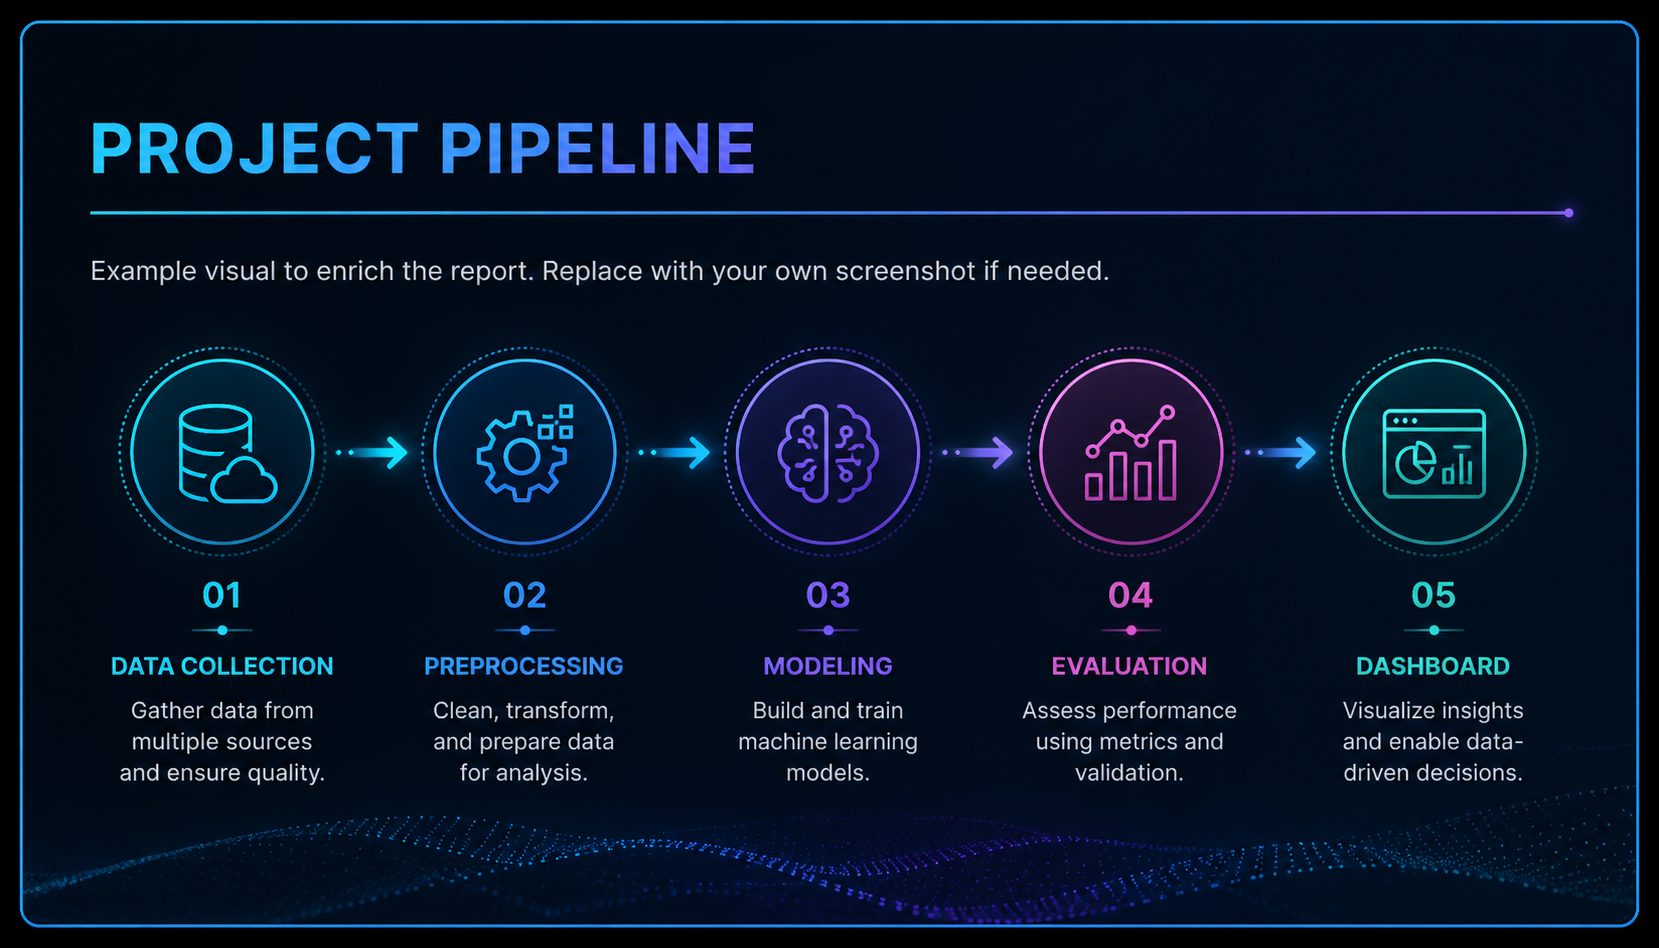
\includegraphics[width=0.85\textwidth]{project_pipeline (2).png}
\caption{Illustrative pipeline of the project workflow.}
\label{fig:pipeline}
\end{figure}

The planning followed an incremental logic.
Early work focused on understanding the data.
Later work concentrated on model comparison and dashboard enhancement.
This progression allowed the project to remain aligned with its objectives while adapting to practical findings.
\section*{Gantt Chart }

\begin{center}
\begin{ganttchart}[
    time slot format=isodate,
    compress calendar,
    x unit=0.7cm,
    y unit chart=0.9cm,
    bar height=0.6,
    vgrid, hgrid,
    bar label font=\small\rmfamily,
    group label font=\bfseries\small,
    title label font=\bfseries\small,
    title/.style={draw=none, fill=none},
    label text width=4cm,
    label text font=\small,
    expand chart=\textwidth
]{2025-02-01}{2025-05-17}

\gantttitlecalendar{month=name}\\

\ganttbar{Problem Analysis}{2025-02-01}{2025-02-10} \\
\ganttbar{Report Writing}{2025-02-11}{2025-02-15} \\
\ganttbar{Requirement Analysis}{2025-02-16}{2025-02-29} \\
\ganttbar{Report Writing}{2025-03-01}{2025-03-05} \\
\ganttbar{System Design}{2025-03-06}{2025-03-20} \\
\ganttbar{Report Writing}{2025-03-21}{2025-03-25} \\
\ganttbar{Implementation}{2025-03-26}{2025-04-15} \\
\ganttbar{Report Writing}{2025-04-16}{2025-04-20} \\
\ganttbar{Testing \& Debugging}{2025-04-21}{2025-05-10} \\
\ganttbar{Report Writing}{2025-05-11}{2025-05-17} \\
\end{ganttchart}

\vspace{0.5em}
\textbf{Figure: Project Timeline }
\end{center}



\begin{table}[H]
\vspace*{\fill}
\centering
\Large
\renewcommand{\arraystretch}{2.0} % increase row height

\caption{Project Schedule}

\begin{tabular}{|p{6cm}|c|c|c|}
\hline
\textbf{Task Name} & \textbf{Start Date} & \textbf{End Date} & \textbf{Duration (days)} \\
\hline
Problem Analysis           & 01-Feb-2025 & 10-Feb-2025 & 10 \\
Report Writing             & 11-Feb-2025 & 15-Feb-2025 & 5  \\
Requirement Analysis       & 16-Feb-2025 & 29-Feb-2025 & 14 \\
Report Writing             & 01-Mar-2025 & 05-Mar-2025 & 5  \\
System Design              & 06-Mar-2025 & 20-Mar-2025 & 15 \\
Report Writing             & 21-Mar-2025 & 25-Mar-2025 & 5  \\
Implementation             & 26-Mar-2025 & 15-Apr-2025 & 21 \\
Report Writing             & 16-Apr-2025 & 20-Apr-2025 & 5  \\
Testing \& Debugging       & 21-Apr-2025 & 10-May-2025 & 20 \\
Report Writing             & 11-May-2025 & 17-May-2025 & 7  \\
\hline
\end{tabular}

\vspace*{\fill}
\end{table}



\section{Analytical Scope of the Project}

The project is built around a clear objective: analyzing the relationship between the United States housing market and macroeconomic indicators while creating a Streamlit dashboard to visualize, compare, predict, and interpret housing-price behavior. This objective is implemented through a complete housing intelligence platform.

The platform includes the following functional blocks:
\begin{itemize}
\item \textbf{OLAP analysis}: multidimensional exploration through pivot tables, grouped metrics, and segmentation.
\item \textbf{AI chatbot}: natural language interaction with the project and its results.
\item \textbf{Prompt chatbot}: structured prompt-based guidance for users who want analytical explanations without coding.
\item \textbf{Unsupervised learning}: K-Means, DBSCAN, PCA, and anomaly detection to discover hidden patterns.
\item \textbf{Reinforcement learning}: an educational decision-policy module that illustrates state, action, reward, and policy logic.
\item \textbf{Paper review and comparison}: comparison between project findings, economic theory, and market-period interpretation.
\item \textbf{Streamlit deployment}: a complete interactive product with navigation, styling, export, and production-readiness checks.
\item \textbf{Model governance}: experiment tracking, model registry, validation checks, and model-card style interpretation.
\end{itemize}

This scope is important because real data science projects rarely stop at a single model. A useful analytical product must also provide interpretation, reproducibility, usability, and decision support. The extended project therefore moves closer to a professional workflow used in companies, banks, consultancies, and public institutions.

\section{Business Value}

The dashboard can support several types of users:
\begin{itemize}
\item \textbf{Students and researchers} can use the platform to understand how machine learning models behave on economic data.
\item \textbf{Real estate analysts} can explore market indicators, compare periods, and interpret housing-price movement.
\item \textbf{Financial institutions} can use the workflow as a prototype for risk monitoring, scenario analysis, and affordability analysis.
\item \textbf{Policy-oriented users} can compare macroeconomic periods and study how housing indicators evolved under different market conditions.
\end{itemize}

The value of the project is therefore not only technical. It is also educational and managerial. It helps transform raw economic data into understandable insight.

\section{CRISP-DM Mapping}

The project still follows CRISP-DM, but each phase now contains additional components.

\begin{longtable}{p{4cm}p{11cm}}
\toprule
\textbf{CRISP-DM phase} & \textbf{Implementation in the project} \\
\midrule
Business Understanding & Definition of the housing market problem, business impact, user needs, and decision-support objectives. \\
Data Understanding & Dataset preview, date detection, numeric profiling, missing-value checks, duplicate checks, and correlation exploration. \\
Data Preparation & Column cleaning, date parsing, numeric conversion, administration labeling, lag features, rolling means, differencing, and imputation. \\
Modeling & Regression, classification, model comparison, forecasting, clustering, PCA, anomaly detection, and reinforcement-learning simulation. \\
Evaluation & MAE, RMSE, R squared, accuracy, precision, recall, F1-score, ROC AUC, clustering quality metrics, and interpretability checks. \\
Deployment & Streamlit dashboard, export modules, AI chatbot, prompt interaction, production-readiness checks, experiment tracking, and model registry. \\
\bottomrule
\caption{Mapping between CRISP-DM and the analytical platform.}
\end{longtable}

\section{Functional Requirements}

The system must satisfy the following functional requirements:
\begin{enumerate}
\item Load a housing and macroeconomic dataset from a default path or user upload.
\item Clean and prepare the dataset automatically.
\item Detect the date column and generate time-based comparisons.
\item Visualize trends, correlations, distributions, and administration-level differences.
\item Train supervised models for regression and classification tasks.
\item Compare several models using standard evaluation metrics.
\item Generate forecasts using lagged and rolling variables.
\item Apply unsupervised learning to discover clusters and anomalies.
\item Provide OLAP-style pivot and segmentation analysis.
\item Offer chatbot and prompt-based assistance for interpretation.
\item Export reports, tables, and insights.
\item Present production-readiness and governance checks.
\end{enumerate}

\section{Non-Functional Requirements}

The platform must also satisfy non-functional requirements:
\begin{itemize}
\item \textbf{Usability}: the dashboard must be understandable to non-technical users.
\item \textbf{Modularity}: the code should be organized into reusable helper functions.
\item \textbf{Reproducibility}: data cleaning, model training, and evaluation steps must be documented.
\item \textbf{Interpretability}: the system should explain why a model or variable is important.
\item \textbf{Scalability}: the design should allow future modules or datasets to be added.
\item \textbf{Reliability}: validation checks should warn the user before trusting weak data or unstable models.
\end{itemize}

\section{Project Contribution}

The project contributes a broad and realistic data science workflow. The contribution can be summarized in four points:
\begin{enumerate}
\item It connects housing-market analysis with macroeconomic interpretation.
\item It combines classical supervised learning with unsupervised learning and reinforcement-learning concepts.
\item It adds an interaction layer through AI and prompt-based assistance.
\item It introduces production-readiness ideas that are often missing in academic dashboards.
\end{enumerate}

This makes the project stronger academically because it demonstrates both technical skills and methodological understanding.

\section{Conclusion}

This chapter introduced the context, problem, objectives, methodology, and technologies of the project. It established the general framework of the study and justified the use of data mining, machine learning, OLAP analysis, AI-assisted interpretation, and interactive deployment for housing market analysis. The chapter also clarified the functional and non-functional requirements that guide the platform design. The next chapter presents the theoretical background required to understand the selected methods in greater detail.


\chapter{State of the Art}
\label{chap:2}

\section{Introduction}

This chapter presents the theoretical background related to data mining, machine learning, regression methods, ensemble models, and data visualization.
It provides the conceptual foundation needed to understand the implementation choices made later in the report.

\section{Data Mining}

Data Mining is the process of extracting relevant information, patterns, and knowledge from raw data.
It lies at the intersection of statistics, machine learning, and database systems.
Its main objective is not only to describe data but also to reveal hidden structures that can support decision-making.

Typical goals of data mining include classification, regression, clustering, anomaly detection, and association analysis.
In economic contexts, data mining is especially useful for understanding relationships between indicators, discovering structural trends, and building predictive systems.

\section{Machine Learning}

Machine Learning is a branch of artificial intelligence that enables systems to learn from examples rather than relying solely on manually written rules.
A machine learning model uses historical data to identify patterns and generalize them to unseen observations.

\subsection{Supervised Learning}

Supervised learning is based on labeled examples.
The model receives input variables and a target output, then learns a mapping between them.
In this project, supervised learning is used to predict a housing-related target variable from macroeconomic indicators.

Regression and classification are the two main supervised learning settings.
Because our objective is numerical prediction, regression is the most relevant family.

\subsection{Unsupervised Learning}

Unsupervised learning works without labeled targets.
Its objective is to identify internal structures in the data, such as clusters or latent dimensions.
Although this project focuses mainly on supervised prediction, unsupervised ideas remain useful in exploratory analysis.

\section{Regression Models}

Regression models estimate the relationship between one dependent variable and one or several explanatory variables.
They are central tools in both statistics and machine learning.

\subsection{Linear Regression}

Linear regression assumes a linear relationship between the predictors and the response:
\[
y = \beta_0 + \beta_1x_1 + \beta_2x_2 + \dots + \beta_px_p + \varepsilon
\]

Its major strength is interpretability.
However, its performance can degrade when predictors are correlated or when the relationship is not sufficiently linear.

\subsection{Ridge Regression}

Ridge Regression extends linear regression by adding an \(L_2\) penalty on the coefficients:
\[
\min_{\beta} \|y - X\beta\|^2 + \lambda \|\beta\|^2
\]

This regularization reduces overfitting and improves stability in the presence of multicollinearity.
For this reason, Ridge Regression is often used as a solid baseline in predictive tasks involving multiple correlated indicators.

\section{Ensemble Learning and Random Forest}

Ensemble learning combines multiple models in order to obtain a more robust final prediction.
Instead of relying on a single learner, it aggregates several models and often improves performance.

Random Forest is one of the most popular ensemble techniques.
It constructs many decision trees using bootstrap samples and random subsets of features.
The final prediction is obtained by averaging the outputs of all trees.

Its main strengths are:
\begin{itemize}
\item the ability to model non-linear relationships,
\item robustness to noise,
\item resistance to overfitting compared with a single decision tree,
\item and an internal measure of feature importance.
\end{itemize}

For economic datasets where variable interactions can be complex, Random Forest is therefore a strong candidate.

\section{Evaluation Metrics}

Model evaluation is a crucial stage in machine learning.
A model should not only fit the training data but also perform well on unseen observations.
In this project, three standard metrics are used.

\subsection{Mean Absolute Error}

Mean Absolute Error measures the average absolute difference between predicted and observed values:
\[
MAE = \frac{1}{n}\sum_{i=1}^{n} |y_i - \hat{y}_i|
\]

It is easy to interpret and less sensitive to large errors than squared measures.

\subsection{Root Mean Squared Error}

Root Mean Squared Error is defined by:
\[
RMSE = \sqrt{\frac{1}{n}\sum_{i=1}^{n}(y_i - \hat{y}_i)^2}
\]

Because it squares the errors before averaging, it penalizes large deviations more strongly than MAE.

\subsection{Coefficient of Determination}

The coefficient of determination is written as:
\[
R^2 = 1 - \frac{SS_{res}}{SS_{tot}}
\]

It measures the proportion of variance explained by the model.
A value closer to 1 indicates better explanatory power.

\section{Exploratory Data Analysis and Visualization}

Exploratory Data Analysis, often abbreviated as \gls{eda}, is a preliminary stage in which the analyst investigates the dataset through summary statistics and visual representations.
This stage is fundamental because it helps identify missing values, abnormal observations, variable distributions, and potential relationships.

Visualization is not just decorative.
It is a cognitive tool that makes complex patterns easier to understand.
Time series plots, correlation matrices, box plots, and comparative charts allow the analyst to move from raw data to interpretable structure.

\section{Dashboards and Interactive Analytics}

A dashboard is an interface that gathers visual components and filters into a single environment.
In data science projects, dashboards play an important role because they connect technical analysis with practical usability.

In this project, Streamlit was selected as the dashboard framework.
It makes it possible to transform Python code into an interactive web application quickly.
Users can inspect variables, filter data, compare periods, and display predictions without editing the underlying code.

\begin{figure}[H]
\centering
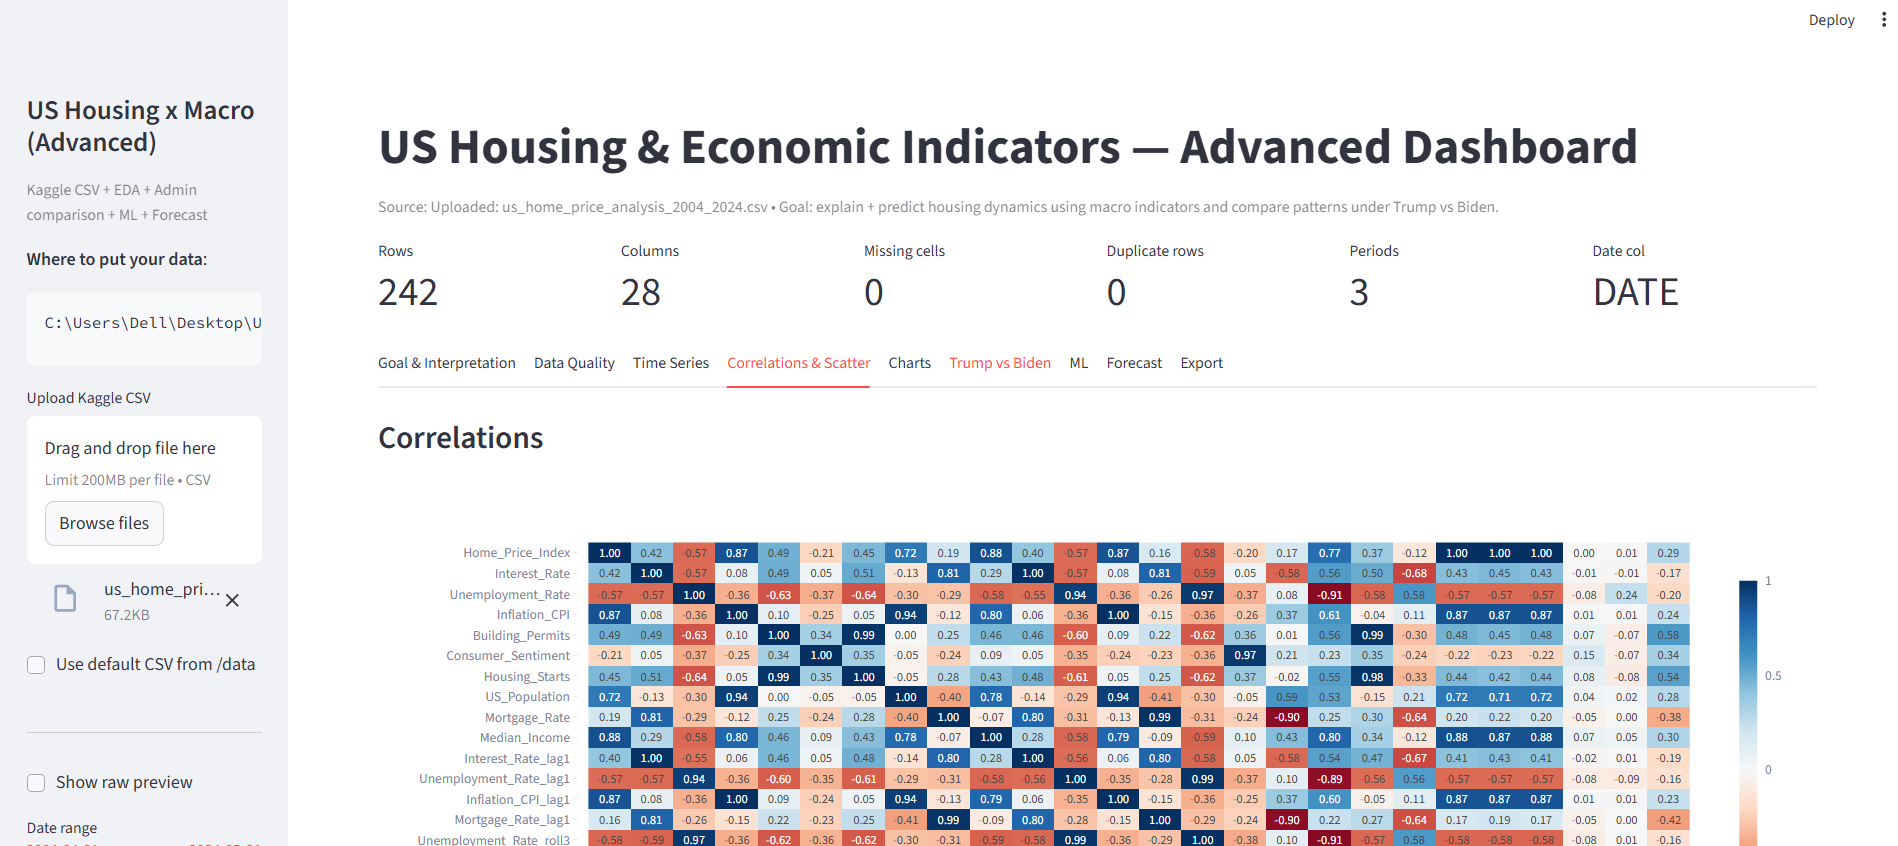
\includegraphics[width=0.82\textwidth]{dashboard_placeholder.png}
\caption{Example placeholder for the dashboard overview. Replace with a real screenshot if available.}
\label{fig:dashboard}
\end{figure}

\section{Applications in Housing Market Analysis}

The housing market has been widely studied using both classical econometric tools and modern machine learning methods.
Researchers and analysts often use explanatory variables such as mortgage rates, income, inflation, and unemployment to understand real estate dynamics.

Machine learning methods are especially useful when the goal is to combine many indicators, uncover non-linear interactions, and build predictive systems that can be refreshed as new data becomes available.
This makes them particularly relevant for dashboards and decision-support tools.

\section{Conclusion}

This chapter reviewed the theoretical concepts underlying the project.
It explained the principles of data mining and machine learning, introduced regression and ensemble methods, and emphasized the role of visualization and dashboards in analytical workflows.
These concepts serve as the basis for the implementation chapter, where the concrete system design and development choices are presented.

\section{OLAP and Multidimensional Analysis}

Online Analytical Processing, usually abbreviated as OLAP, refers to analytical techniques that allow users to examine data across several dimensions. In classical business intelligence, OLAP is used to create summaries such as sales by region, profit by product category, or customer behavior by period. In this project, the same logic is applied to housing and macroeconomic indicators.

The purpose of OLAP in the project is not to replace machine learning. Instead, OLAP complements machine learning by making the data easier to interpret. A predictive model may produce a strong score, but decision-makers often need to understand how averages, medians, changes, and distributions differ across periods or groups.

\subsection{OLAP Operations}

Several OLAP concepts are relevant to the project:
\begin{itemize}
\item \textbf{Roll-up}: aggregation from detailed observations to higher-level summaries, such as monthly values grouped by administration period.
\item \textbf{Drill-down}: movement from an aggregated view to a more detailed view, for example from average housing prices to monthly evolution.
\item \textbf{Slice}: selection of one specific dimension value, such as analyzing only the Biden period.
\item \textbf{Dice}: filtering the data using several dimensions at the same time, such as selecting a period and a set of economic variables.
\item \textbf{Pivot}: rotating dimensions to compare metrics in a table format.
\end{itemize}

\section{AI Chatbots in Data Science Applications}

An AI chatbot is an interface that allows users to interact with a system using natural language. In a data science project, this is useful because many users do not know how to write Python code or interpret model metrics. The chatbot can help explain results, summarize findings, and guide the user toward relevant dashboard pages.

In the project, the chatbot layer is connected to the idea of analytical accessibility. Instead of forcing the user to understand all technical components directly, the system can answer questions such as:
\begin{itemize}
\item What is the strongest driver of housing prices?
\item Which model performed best?
\item What does RMSE mean?
\item Why are lag features useful for forecasting?
\item How should I interpret the OLAP comparison?
\end{itemize}

\section{Prompt Engineering and Prompt Chatbot}

Prompt engineering is the practice of writing clear instructions that guide an AI system toward useful answers. In the context of this project, prompt-based interaction is used to help users formulate analytical questions.

A prompt chatbot differs from a simple chatbot because it can structure the user's request. For example, instead of only answering a vague question, the prompt system can guide the user to specify:
\begin{itemize}
\item the target variable,
\item the period of interest,
\item the model to evaluate,
\item the type of explanation needed,
\item and the business context of the question.
\end{itemize}

This is important because good data analysis depends on good questions. A weak question often produces a weak interpretation, while a precise prompt can lead to a useful analytical answer.

\section{Unsupervised Learning}

Unsupervised learning refers to machine learning methods that do not require labeled output variables. Instead of predicting a known target, these methods search for hidden structure in the data. In housing market analysis, unsupervised learning can help identify similar periods, detect unusual observations, or reduce the dimensionality of the dataset.

\subsection{K-Means Clustering}

K-Means clustering groups observations into a predefined number of clusters. Each cluster contains observations that are similar according to selected numerical features. In this project, K-Means can be used to group months or periods with similar macroeconomic profiles.

\subsection{DBSCAN}

DBSCAN is a density-based clustering method. Unlike K-Means, it does not require all observations to belong to compact spherical clusters. It can also identify noise points. This is useful when the housing market contains abnormal periods, such as crisis months or unusual macroeconomic shocks.

\subsection{Principal Component Analysis}

Principal Component Analysis, or PCA, transforms correlated variables into a smaller set of components. The objective is to reduce dimensionality while preserving as much information as possible. PCA is useful for visualization because complex economic datasets often contain many correlated indicators.

\subsection{Isolation Forest}

Isolation Forest is an anomaly detection method. It isolates observations that are different from the majority of the data. In the housing-market context, anomalies can represent abnormal combinations of prices, interest rates, unemployment, or inflation.

\section{Reinforcement Learning}

Reinforcement learning is a machine learning paradigm in which an agent learns by interacting with an environment. The agent observes a state, chooses an action, receives a reward, and updates its policy. In this project, reinforcement learning is used as an educational module rather than as the main predictive engine.

The main concepts are:
\begin{itemize}
\item \textbf{State}: a representation of the current situation.
\item \textbf{Action}: a decision available to the agent.
\item \textbf{Reward}: feedback that evaluates the quality of the action.
\item \textbf{Policy}: a strategy that maps states to actions.
\end{itemize}

For housing analysis, a simplified example can involve actions such as hold, buy, or wait, depending on whether market indicators suggest upward pressure, affordability stress, or uncertainty. The objective is not to provide financial advice, but to demonstrate how decision policies can be formalized.

\section{Experiment Tracking and Model Registry}

Professional data science requires more than training a single model. Analysts need to know which model was trained, with which features, using which parameters, and with which results. Experiment tracking records these details and supports reproducibility.

A model registry is a structured place where candidate models are stored and compared. It helps identify a champion model, document evaluation results, and prepare for deployment. In the project, these concepts are represented through dashboard modules that track model performance and governance information.

\section{Production Readiness}

Production readiness refers to the checks required before using a data science system in a real environment. A model may perform well in a notebook but still fail in production if the data changes, if missing values appear, or if the model is not monitored.

Important production-readiness checks include:
\begin{itemize}
\item dataset validity,
\item missing-value monitoring,
\item duplicate detection,
\item feature drift,
\item model-card documentation,
\item explainability,
\item and safe interpretation of predictions.
\end{itemize}

This theoretical background supports the implementation described in the next chapter.


\chapter{System Design and Implementation}
\label{chap:3}

\section{Introduction}

This chapter describes the practical implementation of the proposed solution.
It presents the dataset structure, the preprocessing workflow, the feature engineering strategy, the machine learning pipeline, and the design of the interactive Streamlit dashboard.

\section{Business Understanding}

The business objective of the project is to support a better understanding of housing market dynamics in the United States.
The analytical objective is to learn the relationship between macroeconomic variables and a housing-related target variable, then use that relationship to estimate future trends.

The practical outcome expected from the project is not only a predictive model, but also an application that allows users to inspect data and interpret results visually.

\section{Dataset Presentation}

The dataset used in this project contains a date column and several numerical indicators related to housing and macroeconomic conditions.
Although exact variable names may depend on the source file, the dataset generally includes a housing price metric together with economic features such as inflation, unemployment, and interest rates.

The first step was to inspect the structure of the data:
\begin{itemize}
\item identify the date column,
\item verify numerical columns,
\item detect missing values,
\item and evaluate duplicate observations.
\end{itemize}

\section{Data Preparation}

\subsection{Date Parsing}

Because the project includes a strong time-series component, parsing the date column correctly was essential.
The date variable was converted into a valid datetime format and the dataset was sorted chronologically.

\subsection{Numeric Conversion}

All features expected to be numerical were converted explicitly.
This step reduced the risk of hidden formatting issues and ensured that the models could process the variables correctly.

\subsection{Missing Values}

Missing values are common in real datasets.
Instead of removing every incomplete row, the project used imputation strategies in the machine learning pipeline.
Median imputation was selected because it is simple, robust, and appropriate for many economic indicators.

\subsection{Filtering and Data Quality Checks}

The dashboard also includes data quality indicators such as:
\begin{itemize}
\item number of rows,
\item number of columns,
\item total missing cells,
\item duplicate rows,
\item number of detected periods.
\end{itemize}

These checks provide immediate feedback to the user before advanced analysis begins.

\section{Feature Engineering}

Feature engineering improves the quality of the information provided to the models.
In this project, two forms of feature engineering were especially important.

\subsection{Administrative Period Labeling}

A categorical variable called \textit{administration} was derived from the date column.
This variable groups observations into periods such as:
\begin{itemize}
\item Pre-Trump,
\item Trump (2017--2020),
\item Biden (2021--2024),
\item Post-Biden.
\end{itemize}

This feature helps compare economic and housing behavior across political periods.

\subsection{Lag and Rolling Features}

For forecasting, lagged variables and rolling averages were created.
Examples include:
\begin{itemize}
\item target lag at 1, 3, 6, and 12 periods,
\item rolling means,
\item first differences,
\item lagged explanatory variables.
\end{itemize}

These engineered features make the forecasting stage more informative because they capture temporal dependence.

\section{Dashboard Architecture}

The dashboard was developed with Streamlit and divided into several tabs.
This structure improves navigation and keeps related analyses together.

The main tabs include:
\begin{enumerate}
\item Goal and interpretation,
\item Data quality,
\item Time series,
\item Correlations and scatter plots,
\item Charts,
\item Trump vs Biden comparison,
\item Machine Learning,
\item Forecast,
\item Export.
\end{enumerate}

\subsection{Overview and Interpretation}

The first tab introduces the project objective and highlights the most correlated variables with the selected target.
This gives the user an immediate analytical summary.

\subsection{Data Quality}

The second tab focuses on missing values and general dataset structure.
This is important because users should understand the limitations of the data before trusting any prediction.

\subsection{Time Series Analysis}

A dedicated time series tab allows the visualization of the selected metric through time.
Rolling means can be added to smooth the evolution and highlight long-term trends.

\subsection{Correlation and Scatter Analysis}

The dashboard includes a correlation matrix for all numerical features.
It also allows users to choose two variables and visualize their relationship in a scatter plot with a trend line.
This makes the investigation of pairwise relationships much more intuitive.

\subsection{Distribution and Comparative Charts}

Box plots and violin plots are used to compare distributions across administrations.
This is useful for seeing whether one period systematically differs from another.

\section{Machine Learning Pipeline}

The machine learning module is designed to let the user choose:
\begin{itemize}
\item the target variable,
\item the explanatory features,
\item the scaling method,
\item and the model type.
\end{itemize}

The main steps of the pipeline are:
\begin{enumerate}
\item median imputation,
\item optional scaling,
\item model fitting,
\item test set prediction,
\item metric computation.
\end{enumerate}

\subsection{Selected Models}

Two models were selected:
\begin{itemize}
\item Ridge Regression, as an interpretable regularized baseline,
\item Random Forest, as a flexible ensemble method with stronger capacity to capture non-linear relationships.
\end{itemize}

\subsection{Train/Test Split}

The dataset is divided into training and testing subsets.
A chronological split is used instead of a random split in order to preserve the time order of the observations.
This is more appropriate for economic and temporal data.

\subsection{Performance Metrics}

The model results are summarized using MAE, RMSE, and \(R^2\).
These three metrics provide complementary perspectives:
MAE measures average absolute error, RMSE gives greater importance to large errors, and \(R^2\) evaluates explained variance.

\section{Forecasting Logic}

The forecasting tab extends the analytical value of the project.
A future horizon can be selected, and the target variable is projected step by step.
At each step, lag features and rolling statistics are recalculated so that the model can generate the next value.

Although this forecasting logic remains relatively simple compared with specialized time-series models, it is pedagogically useful and integrates well into the dashboard.

\section{Deployment}

The final system was deployed as a Streamlit application.
This deployment choice is well suited to the project because it transforms code into a user-friendly interface with minimal overhead.
The application can be launched locally and adapted easily if new variables or visualizations are added later.

\section{Conclusion}

This chapter presented the design and implementation of the complete solution.
It described how the data was prepared, how features were engineered, how the machine learning pipeline was structured, and how the dashboard was organized.
The next chapter presents the obtained results and discusses their interpretation.

\section{Application Architecture}

The application is implemented as a Streamlit dashboard that acts as the main entry point of the project. The code is organized around helper functions for data preparation, visualization, modeling, evaluation, reporting, and interface rendering. This architecture makes the application easier to maintain than a single block of procedural code.

\begin{figure}[H]
\centering
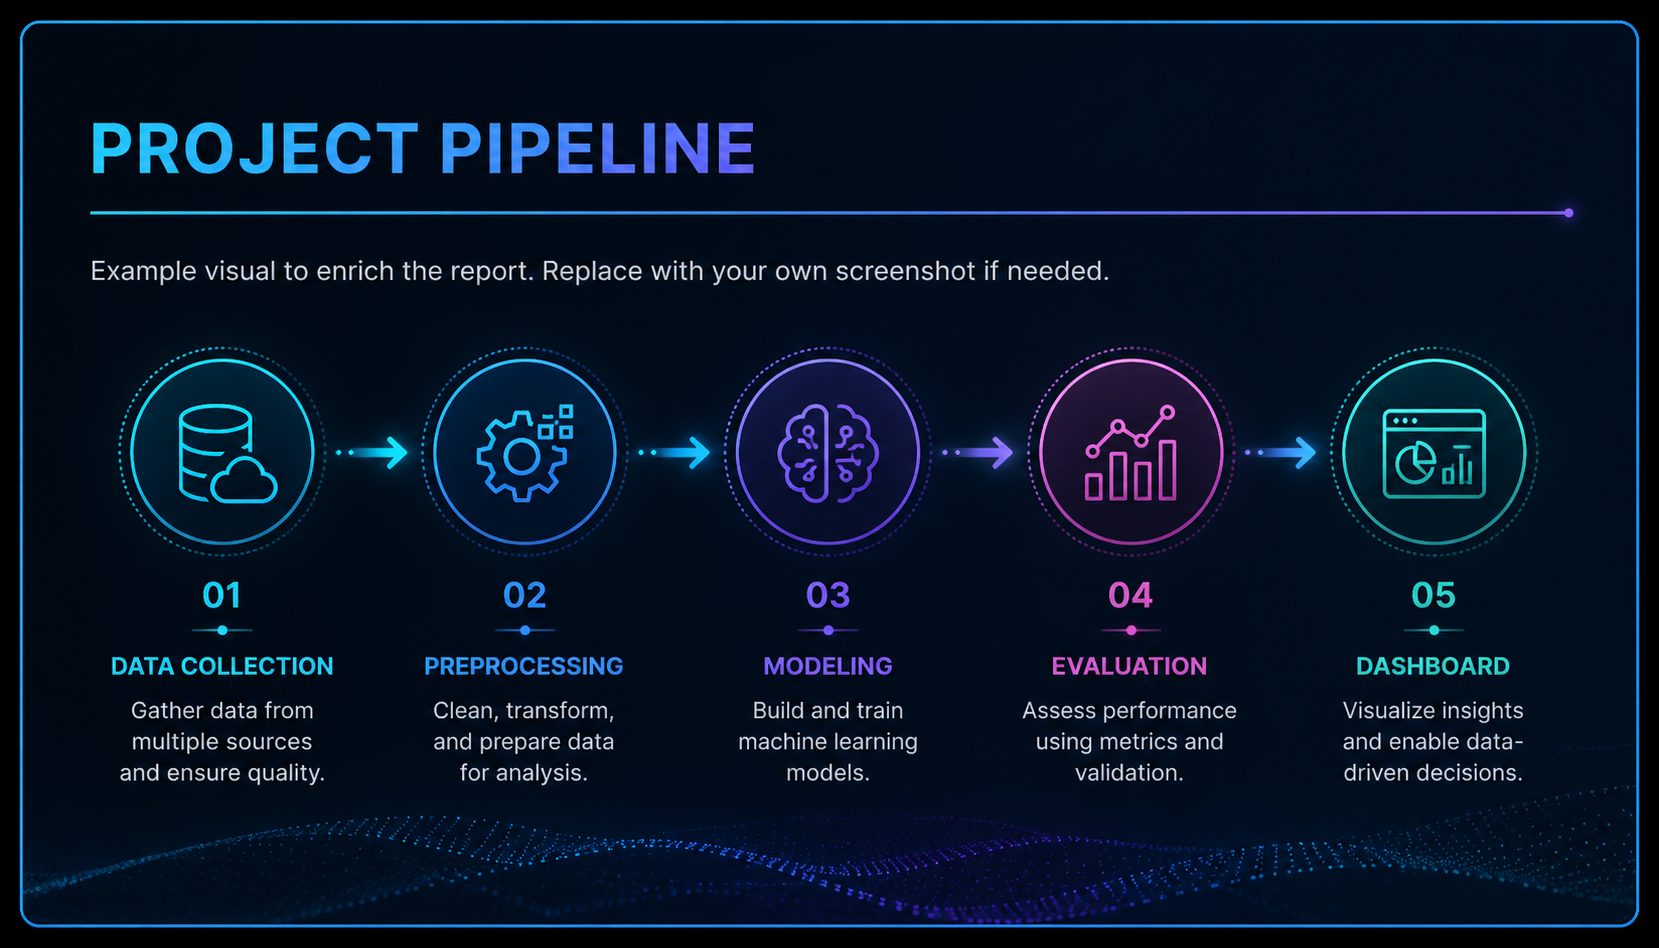
\includegraphics[width=0.95\textwidth]{project_pipeline (2).png}
\caption{End-to-end project pipeline from data loading to interpretation and deployment.}
\label{fig:project_pipeline}
\end{figure}

\subsection{Navigation Structure}

The dashboard navigation is organized to guide the user from general understanding to technical analysis and business interpretation. It contains pages for goal interpretation, data quality, time series, correlations, charts, administration comparison, machine learning, forecasting, export, and analytical pages such as:
\begin{itemize}
\item Overview,
\item Explore,
\item Data Quality,
\item ML Lab,
\item Evaluation,
\item Unsupervised Lab,
\item Reinforcement Lab,
\item Forecast,
\item OLAP and Export,
\item Scenario Simulator,
\item Paper Review,
\item Production Readiness,
\item Experiment Tracker,
\item Model Registry,
\item Data Pipeline,
\item Business Impact.
\end{itemize}

This expanded structure allows the project to cover the complete lifecycle of a data science product.

\section{Data Cleaning Module}

The application includes a documented data cleaning report. The objective is to show not only that the data was cleaned, but also what exactly was checked. The cleaning report includes column-name cleanup, date parsing, numeric conversion, missing-value checks, duplicate-row checks, period feature creation, and row preservation.

\begin{longtable}{p{4cm}p{5cm}p{5cm}}
\toprule
\textbf{Cleaning step} & \textbf{Purpose} & \textbf{Project value} \\
\midrule
Column-name cleanup & Remove leading and trailing spaces & Avoid hidden errors in feature selection. \\
Date parsing & Convert date column into datetime format & Enable chronological sorting and forecasting. \\
Numeric conversion & Convert numeric-looking text into numbers & Make features usable by models. \\
Missing-value check & Count missing cells before and after cleaning & Document data quality. \\
Duplicate-row check & Detect repeated observations & Prevent biased summaries. \\
Period feature creation & Add administration labels & Enable political-period comparison. \\
Row preservation & Verify that cleaning did not remove data unintentionally & Improve reproducibility. \\
\bottomrule
\caption{Data cleaning report logic.}
\end{longtable}

\section{Supervised Learning Module}

The supervised learning module includes a model laboratory. The application supports regression and classification modes and allows the user to compare several algorithms.

\subsection{Regression Models}

The regression models include Ridge Regression, Random Forest Regressor, Linear Regression, Support Vector Regressor, Gradient Boosting Regressor, Decision Tree Regressor, K-Nearest Neighbors Regressor, and Neural Network Regressor.

\subsection{Classification Models}

For classification, the numerical target can be transformed into categories such as low, medium, and high. The classification models include Random Forest Classifier, Logistic Regression, Decision Tree Classifier, K-Nearest Neighbors Classifier, and Neural Network Classifier.

\subsection{Pipeline Design}

The supervised learning pipeline follows this sequence:
\begin{enumerate}
\item Select target and features.
\item Remove rows with missing target values.
\item Split the dataset chronologically into training and testing subsets.
\item Impute missing feature values using the median.
\item Apply optional scaling using StandardScaler or MinMaxScaler.
\item Train the selected model.
\item Predict the test set.
\item Evaluate performance.
\item Display metrics and visual comparison.
\end{enumerate}

\section{Model Evaluation Module}

The evaluation page compares several models under the same conditions. This is important because a single model score is not enough to justify a modeling decision. The dashboard calculates regression metrics such as MAE, RMSE, and R squared, and classification metrics such as accuracy, precision, recall, F1-score, and ROC AUC when available.

\begin{longtable}{p{3cm}p{5cm}p{6cm}}
\toprule
\textbf{Metric} & \textbf{Used for} & \textbf{Interpretation} \\
\midrule
MAE & Regression & Average absolute prediction error. Lower is better. \\
RMSE & Regression & Penalizes large errors more strongly. Lower is better. \\
R squared & Regression & Share of variance explained by the model. Higher is better. \\
Accuracy & Classification & Share of correct predictions. Higher is better. \\
Precision & Classification & Reliability of positive predictions. Higher is better. \\
Recall & Classification & Ability to detect true positive cases. Higher is better. \\
F1-score & Classification & Balance between precision and recall. Higher is better. \\
ROC AUC & Classification & Ranking quality across classes. Higher is better. \\
\bottomrule
\caption{Evaluation metrics used in the dashboard.}
\end{longtable}

\section{Unsupervised Learning Module}

The unsupervised learning page adds exploratory intelligence beyond the supervised target. Its objective is to discover structures that may not be visible in standard charts.

\subsection{K-Means Implementation}

The user selects numerical features and a number of clusters. The features are scaled, the K-Means algorithm is fitted, and the resulting cluster labels are visualized. This helps identify groups of months or observations with similar economic profiles.

\subsection{DBSCAN Implementation}

DBSCAN is used to identify dense regions and outliers. It is particularly useful for detecting unusual market periods. The user can adjust parameters such as neighborhood size and minimum samples.

\subsection{PCA Visualization}

PCA reduces the selected features to principal components. The first two components can be plotted to visualize the structure of the dataset. PCA also helps understand whether the dataset contains strong dominant dimensions.

\subsection{Anomaly Detection}

Isolation Forest identifies observations that are statistically unusual compared with the majority of the data. In housing analysis, such observations may correspond to crisis periods, high-rate shocks, or abnormal combinations of macroeconomic indicators.

\section{Reinforcement Learning Module}

The reinforcement-learning page is an educational module. It illustrates how a decision-making agent can learn from rewards. The module is not intended to provide investment recommendations; instead, it demonstrates the concepts of state, action, reward, and policy.

A simplified housing-market state can be based on indicators such as price trend, interest-rate pressure, and unemployment behavior. Possible actions can include conservative decision labels such as wait, monitor, or act. The reward function evaluates whether the chosen action was suitable under the simulated environment.

\section{OLAP and Export Module}

The OLAP module allows the user to build summarized views of the dataset. The most important OLAP outputs are grouped tables and pivot-style summaries.

Examples of OLAP questions include:
\begin{itemize}
\item What is the average housing price index by administration period?
\item Which period has the highest mean mortgage rate?
\item How do unemployment and inflation compare across periods?
\item Which indicators changed the most between Trump and Biden periods?
\end{itemize}

The export functionality allows users to download relevant tables. This is useful for reports, presentations, and further analysis.

\section{Scenario Simulator}

The scenario simulator is designed for what-if analysis. It allows the user to modify feature values and observe the expected effect on the model output. This helps transform the dashboard from a passive reporting tool into an interactive decision-support system.

Scenario simulation is especially useful in economic analysis because users often ask questions such as:
\begin{itemize}
\item What happens if mortgage rates increase?
\item What happens if unemployment rises?
\item How sensitive is the target to inflation?
\item Which feature change produces the strongest predicted movement?
\end{itemize}

\section{AI Chatbot and Prompt Chatbot Implementation}

The code contains optional OpenAI integration. The application is designed to run even when the OpenAI package or API key is not available. This makes the system robust: users can still use the dashboard without chatbot access, while users with a valid configuration can activate AI assistance.

The chatbot supports natural language interaction. The prompt chatbot complements it by guiding users toward structured analytical questions. This is useful for non-technical users who need explanations of data science outputs.

\section{Paper Review and Real-Market Comparison Module}

The paper review page connects the application results with economic theory and real-world housing-market periods. Instead of presenting machine learning as a black-box exercise, the project compares the dataset behavior with expectations from housing economics.

The module includes theory checks based on expected correlation signs, real-life period comparison, final conclusion generation, and interpretation of why some relationships support or challenge theory.

\section{Production Readiness Module}

The production-readiness page introduces practical checks that would be necessary before deploying a data science product in a professional environment. These checks include dataset validity, missingness, duplicates, date-column availability, target availability, and model governance notes.

This module is important because it shows that the project is not only an academic experiment. It considers how the system could be maintained and monitored in real use.

\section{Experiment Tracker and Model Registry}

The experiment tracker records model runs and their metrics. This allows users to compare experiments over time. The model registry identifies the best candidate model and documents whether it can be promoted as a champion model.

In professional data science, this step is essential because models must be traceable. If a model is used later, the team must know how it was trained, which data was used, and what performance it achieved.

\section{Deployment Logic}

The application is deployed with Streamlit. Streamlit was selected because it allows fast transformation of Python analysis into an interactive web application. The interface includes custom styling with custom styling, sidebar navigation, searchable dashboard destinations, dark/light mode logic, and user-friendly cards.

The deployment workflow is:
\begin{enumerate}
\item Install Python dependencies.
\item Place the dataset in the expected data folder or upload it through the interface.
\item Launch the app using Streamlit.
\item Use the dashboard pages to explore, model, evaluate, export, and interpret results.
\end{enumerate}

\section{Code Organization}

Although the current Streamlit file is the main entry point, the code is written with reusable helper functions. In a future professional implementation, these helpers could be moved into a package such as \texttt{src/us\_housing}. This would separate data preparation, modeling, UI rendering, and reporting logic.

\begin{table}[H]
\centering
\begin{tabularx}{\textwidth}{lX}
\toprule
\textbf{Code component} & \textbf{Role} \\
\midrule
Data helpers & Detect dates, clean data, build reports, calculate correlations. \\
UI helpers & Render metric cards, learning cards, search results, and dashboard layout. \\
Model helpers & Build pipelines, train models, compare algorithms, calculate metrics. \\
Interpretation helpers & Summarize correlations, theory checks, real-life period comparison. \\
Governance helpers & Build data dictionaries, validation reports, executive reports, and model registry outputs. \\
\bottomrule
\end{tabularx}
\caption{Code organization by functional role.}
\end{table}

\section{Conclusion of the Implementation}

The implementation presents a complete housing intelligence platform. It now covers the main pillars of a modern data science product: data preparation, exploratory analysis, supervised learning, unsupervised learning, forecasting, OLAP, chatbot interaction, paper comparison, governance, and deployment.


\chapter{Results and Discussion}
\label{chap:4}

\section{Introduction}

This chapter presents the experimental results of the project.
It discusses the main findings obtained from exploratory data analysis, model training, comparative evaluation, and forecasting.
It also highlights the limitations of the current work and proposes directions for improvement.

\section{Exploratory Findings}

The exploratory analysis revealed that the dataset contains meaningful temporal variation and several potentially informative economic indicators.
The evolution of the housing-related target variable suggested long-term trends as well as period-specific changes.

Correlation analysis showed that some macroeconomic variables are more strongly related to the target than others.
However, correlation alone is not sufficient for prediction, especially when variables interact or when relationships are not purely linear.

Distribution plots by administration also suggested that some economic periods differ more clearly than others.
This supports the idea that contextual or policy-related factors may influence the structure of the housing market.

\section{Model Performance}

The final application compares several regression models under the same chronological train-test logic.
This is more reliable than presenting only one model, because the housing dataset contains strong temporal structure and engineered variables such as lagged values and rolling indicators.
The reproducible evaluation generated from the included CSV is presented later in this chapter in Table~\ref{tab:generated_model_metrics}.

In the generated run, Linear Regression obtains the strongest test result because the dataset includes lagged and smoothed price variables that preserve the main direction of the trend.
This does not mean that Linear Regression is always the best model for housing analysis.
It means that, for this specific feature set, a transparent trend-following model generalizes better to the final chronological period than tree-based models.
The Random Forest and Gradient Boosting results remain useful diagnostic evidence because they show the difficulty of extrapolating a rising market when the test period moves outside the range learned in training.

\section{Feature Importance and Interpretation}

The correlation and diagnostic graphics show that lagged and smoothed price indicators are the strongest predictors in the current dataset.
This is coherent with the housing-market context because home prices usually evolve gradually rather than changing abruptly from one month to the next.
Macroeconomic indicators such as mortgage rates, interest rates, inflation, unemployment, income, building permits, and consumer sentiment remain important for interpretation because they explain the market environment around the price movement.

The main lesson is that predictive strength and economic explanation are not identical.
Lag features may predict very well, but the paper-review and OLAP sections are still needed to explain why the market behaves that way.

\section{Forecast Results}

The forecasting component generated a sequence of future estimated values over a selected horizon.
The projected series remained consistent with the historical trajectory and reflected the persistence captured through lag features.

The forecast should be interpreted carefully.
It is not a guarantee of future market behavior.
Instead, it is a model-based projection under the assumptions embedded in the training data and the chosen feature engineering process.

\section{Dashboard Contribution}

Beyond the numerical metrics, the dashboard is one of the most valuable outcomes of the project.
It transforms the analysis into an interactive environment where users can:
\begin{itemize}
\item inspect data quality,
\item select targets and features,
\item compare periods,
\item visualize distributions,
\item train models,
\item and export results.
\end{itemize}

This practical dimension increases the usefulness of the project and makes the results easier to communicate.

\section{Data-Driven Result Snapshot}

To make the final discussion concrete, the report assets were regenerated from the included CSV file using a chronological 80/20 train-test split. The target variable is \texttt{Home\_Price\_Index}, and the predictors are the remaining numerical macroeconomic and engineered features. This makes the reported results reproducible from the project package.

\begin{figure}[H]
\centering
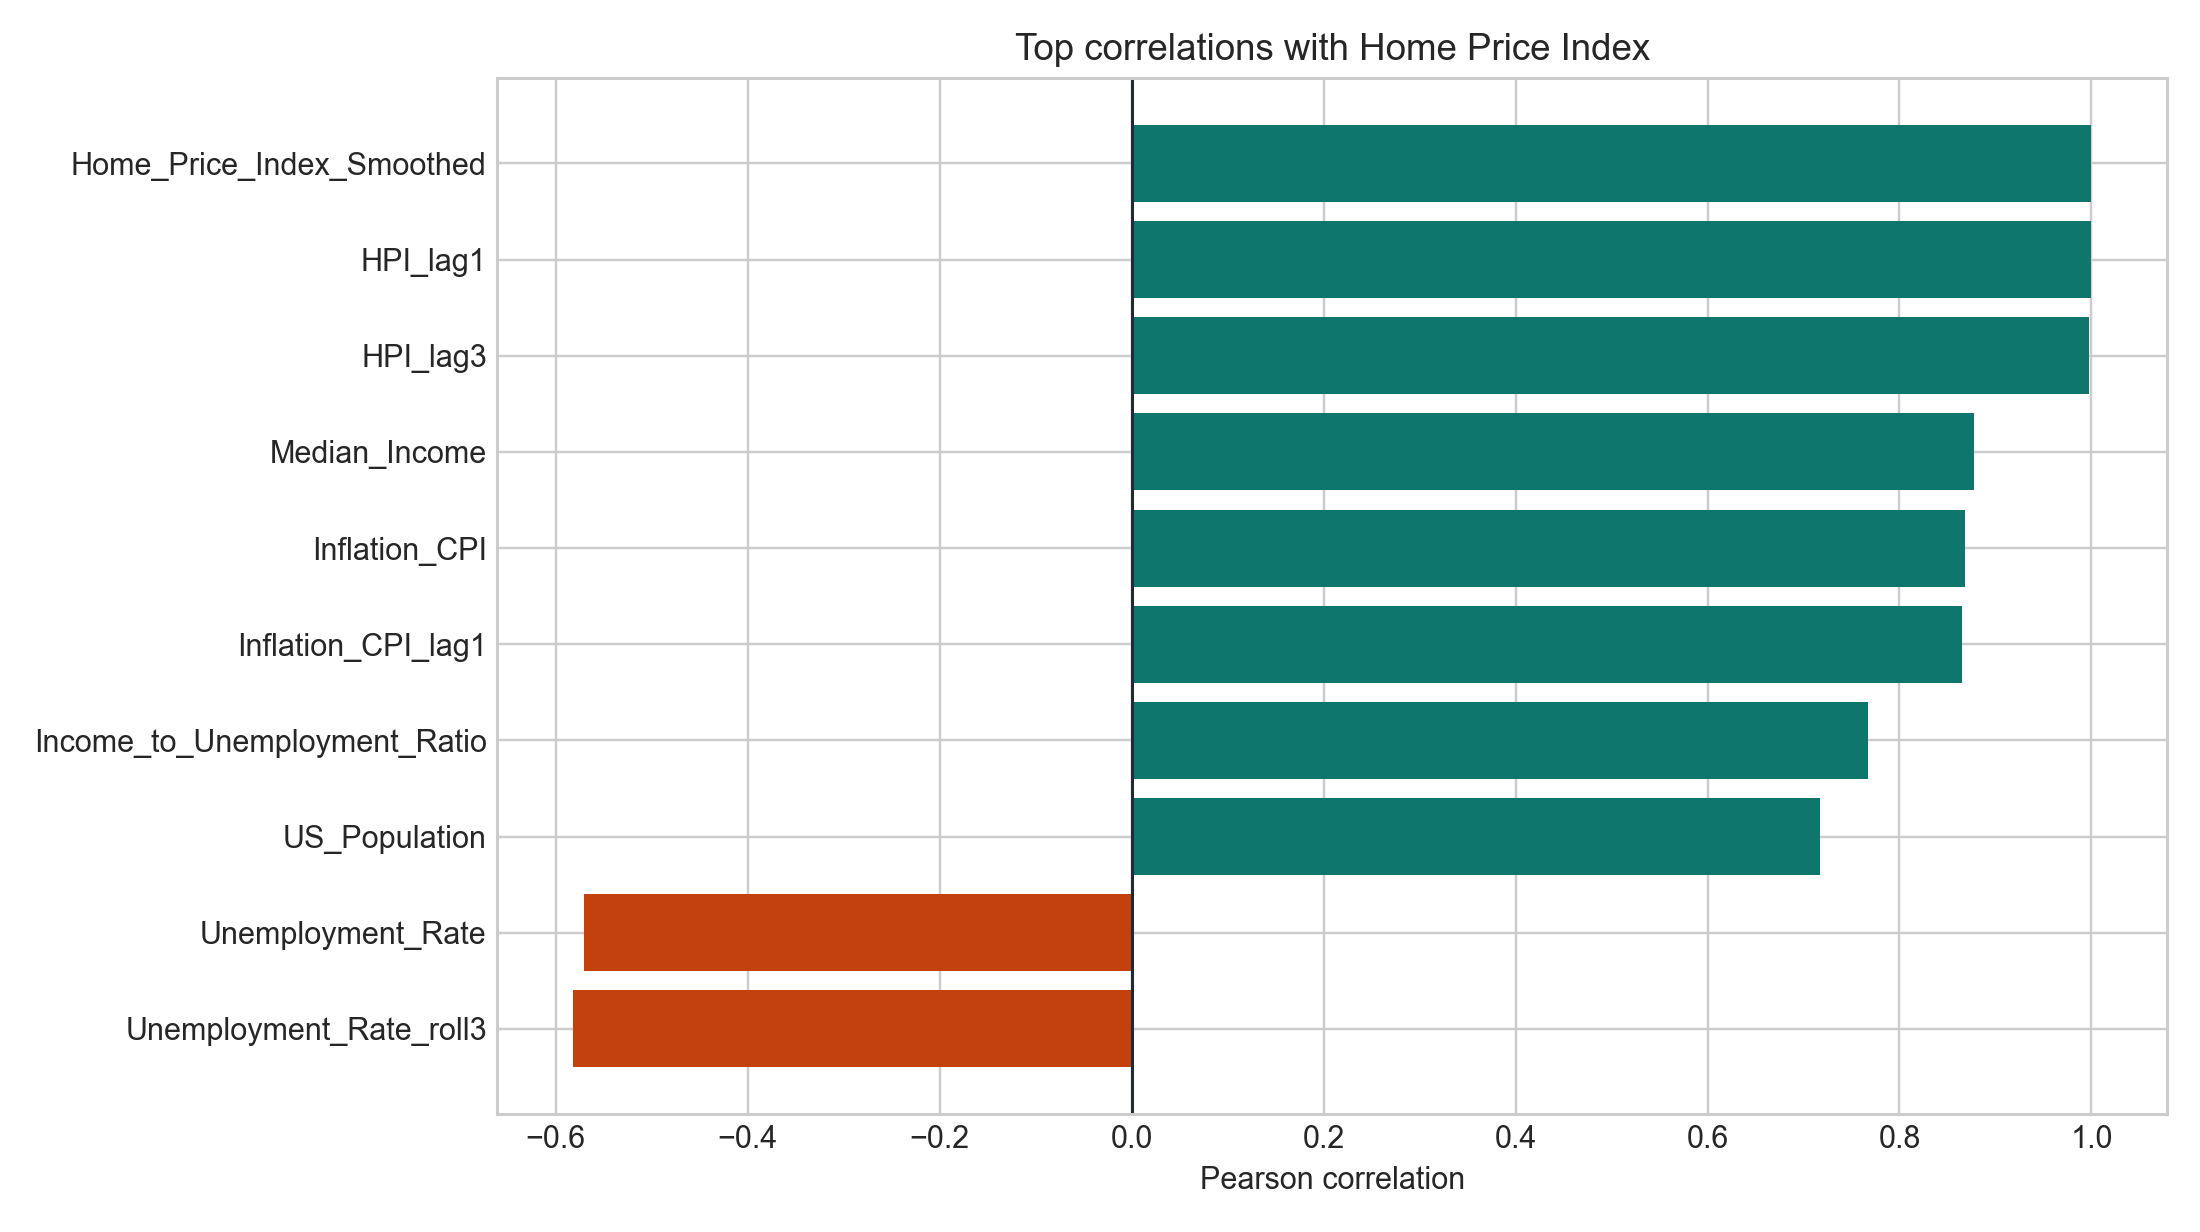
\includegraphics[width=0.92\textwidth]{figures/correlation_results.png}
\caption{Strongest correlations with the Home Price Index in the project dataset.}
\label{fig:generated_corr}
\end{figure}

The strongest linear relationships with the target are: \texttt{Home\_Price\_Index\_Smoothed} (1.00), \texttt{HPI\_lag1} (1.00), \texttt{HPI\_lag3} (1.00), \texttt{Median\_Income} (0.88). These correlations support the paper-review conclusion that housing prices should be interpreted through several linked economic forces, not through a single variable.

\begin{table}[H]
\centering
\begin{tabular}{lrrrr}
\toprule
\textbf{Model} & \textbf{MAE} & \textbf{RMSE} & \textbf{$R^2$} & \textbf{CV $R^2$} \\
\midrule
Linear Regression & 0.661 & 0.797 & 0.999 & 0.994 \\
Ridge Regression & 3.715 & 4.162 & 0.984 & -3.135 \\
Gradient Boosting & 65.816 & 73.669 & -4.148 & -2.458 \\
Decision Tree & 66.218 & 73.750 & -4.159 & -3.315 \\
Random Forest & 69.077 & 76.105 & -4.494 & -2.619 \\
KNN & 74.459 & 79.883 & -5.053 & -4.314 \\
SVR & 103.767 & 109.606 & -10.395 & -7.678 \\
\bottomrule
\end{tabular}
\caption{Generated regression comparison on the chronological test set.}
\label{tab:generated_model_metrics}
\end{table}

The best test-set model in this generated run is \textbf{Linear Regression}, with \(R^2=0.999\), RMSE \(=0.797\), and MAE \(=0.661\). Because the dataset includes lagged and smoothed price features, the linear model can extrapolate the rising trend very effectively. The weaker tree-model scores are also informative: tree ensembles can capture non-linear interactions, but they may struggle when the test period moves beyond the range learned during training.

\begin{figure}[H]
\centering
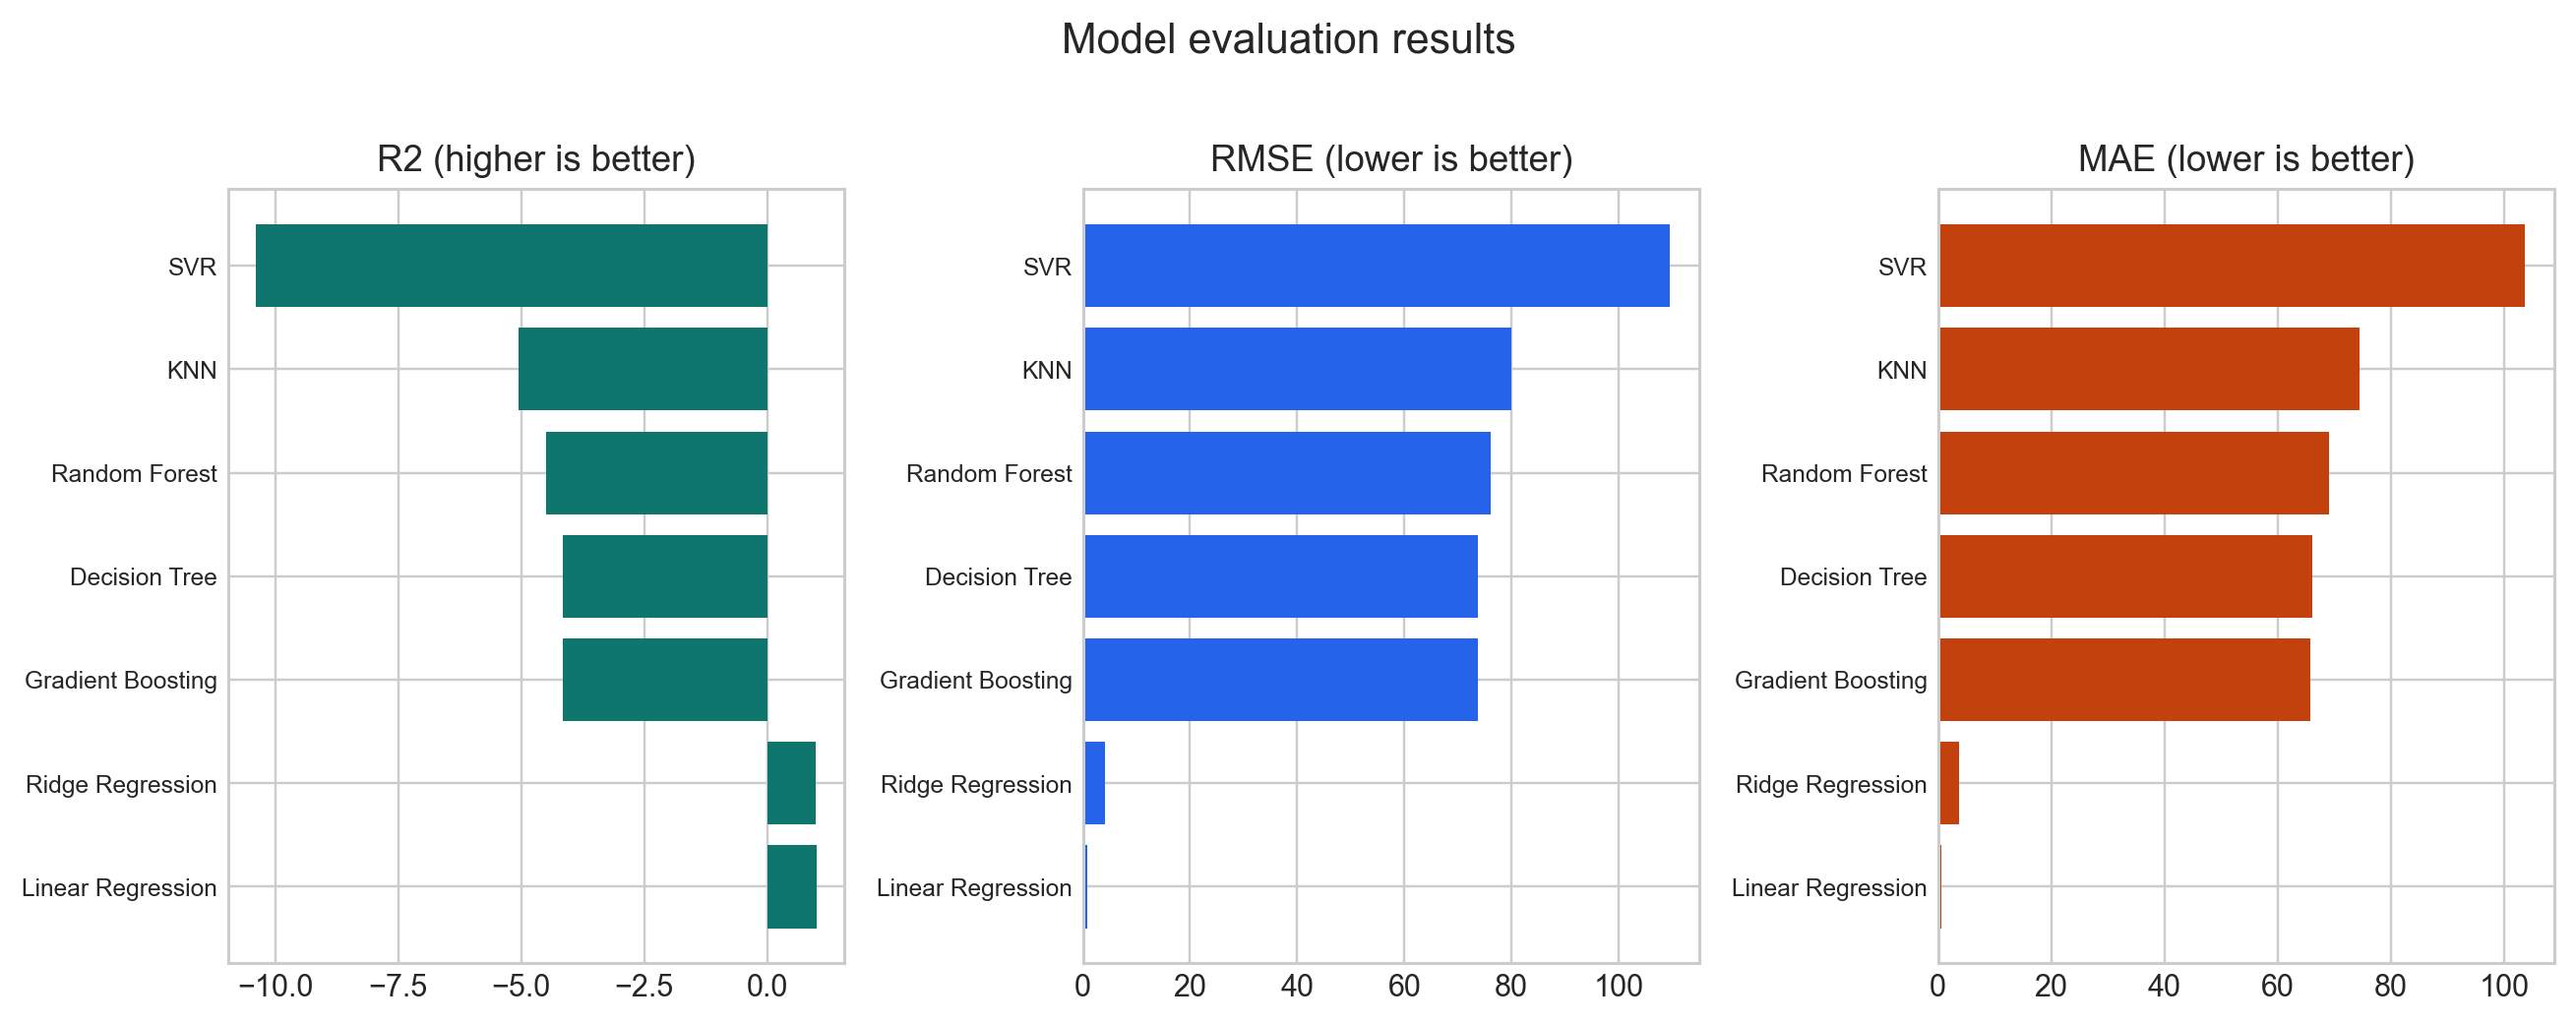
\includegraphics[width=0.98\textwidth]{figures/model_evaluation_results.png}
\caption{Evaluation graphics generated from the model comparison module.}
\label{fig:generated_eval}
\end{figure}

\begin{figure}[H]
\centering
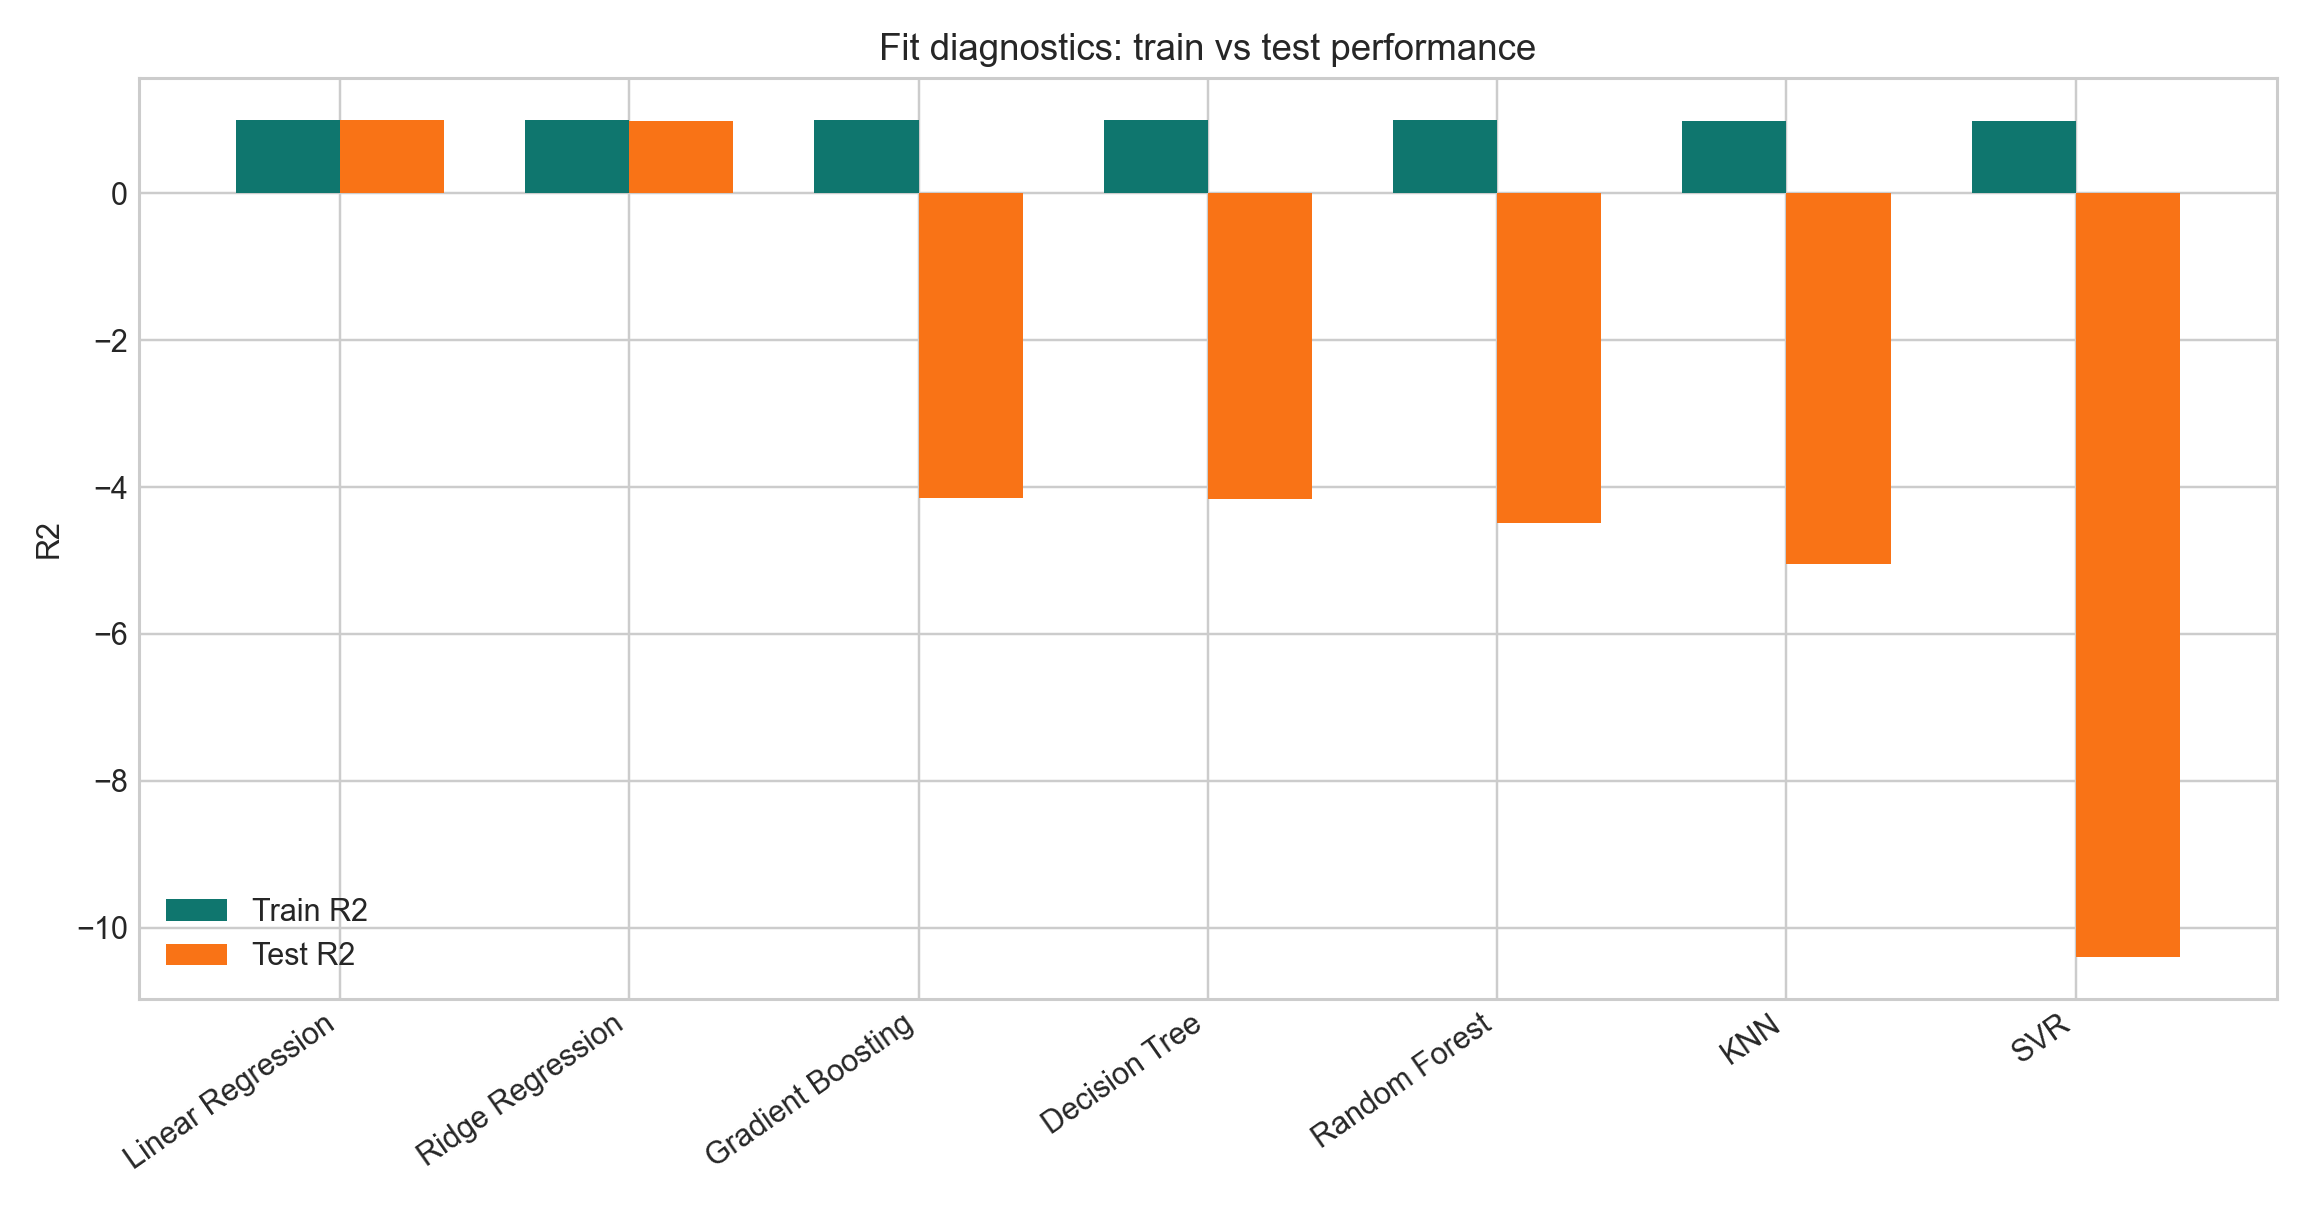
\includegraphics[width=0.92\textwidth]{figures/fit_diagnostics_results.png}
\caption{Fit diagnostics comparing train and test performance.}
\label{fig:generated_diag}
\end{figure}

The diagnostics figure shows whether a model generalizes beyond the training period. A large train-test gap indicates overfitting risk, while a weak score on both sets indicates underfitting. This is why the final project does not rely only on the highest raw score: it also asks whether the result is stable and explainable.

\begin{figure}[H]
\centering
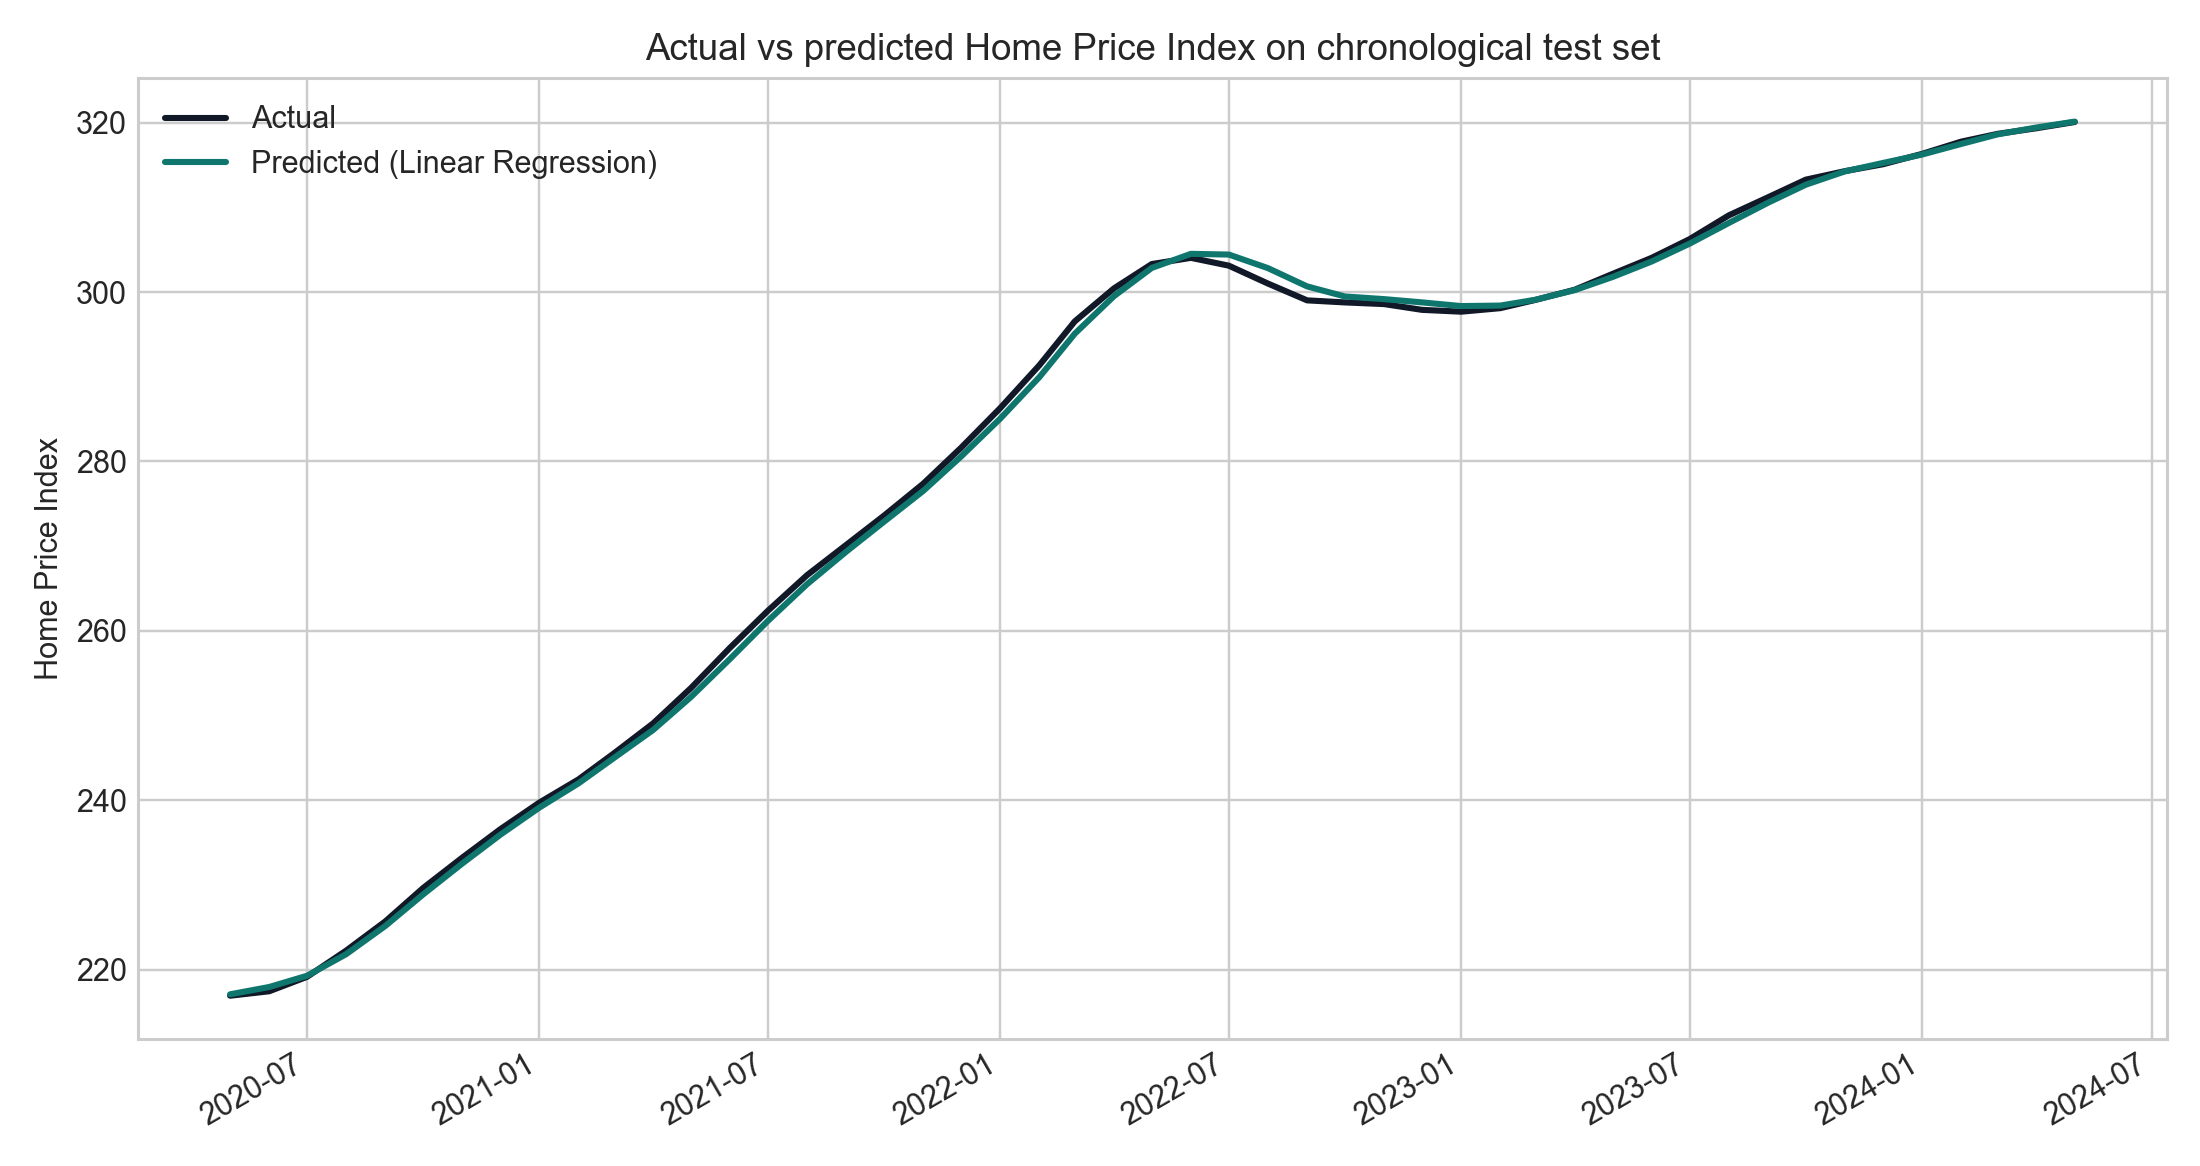
\includegraphics[width=0.92\textwidth]{figures/actual_vs_predicted_results.png}
\caption{Actual and predicted Home Price Index for the best model on the test period.}
\label{fig:generated_pred}
\end{figure}

\begin{figure}[H]
\centering
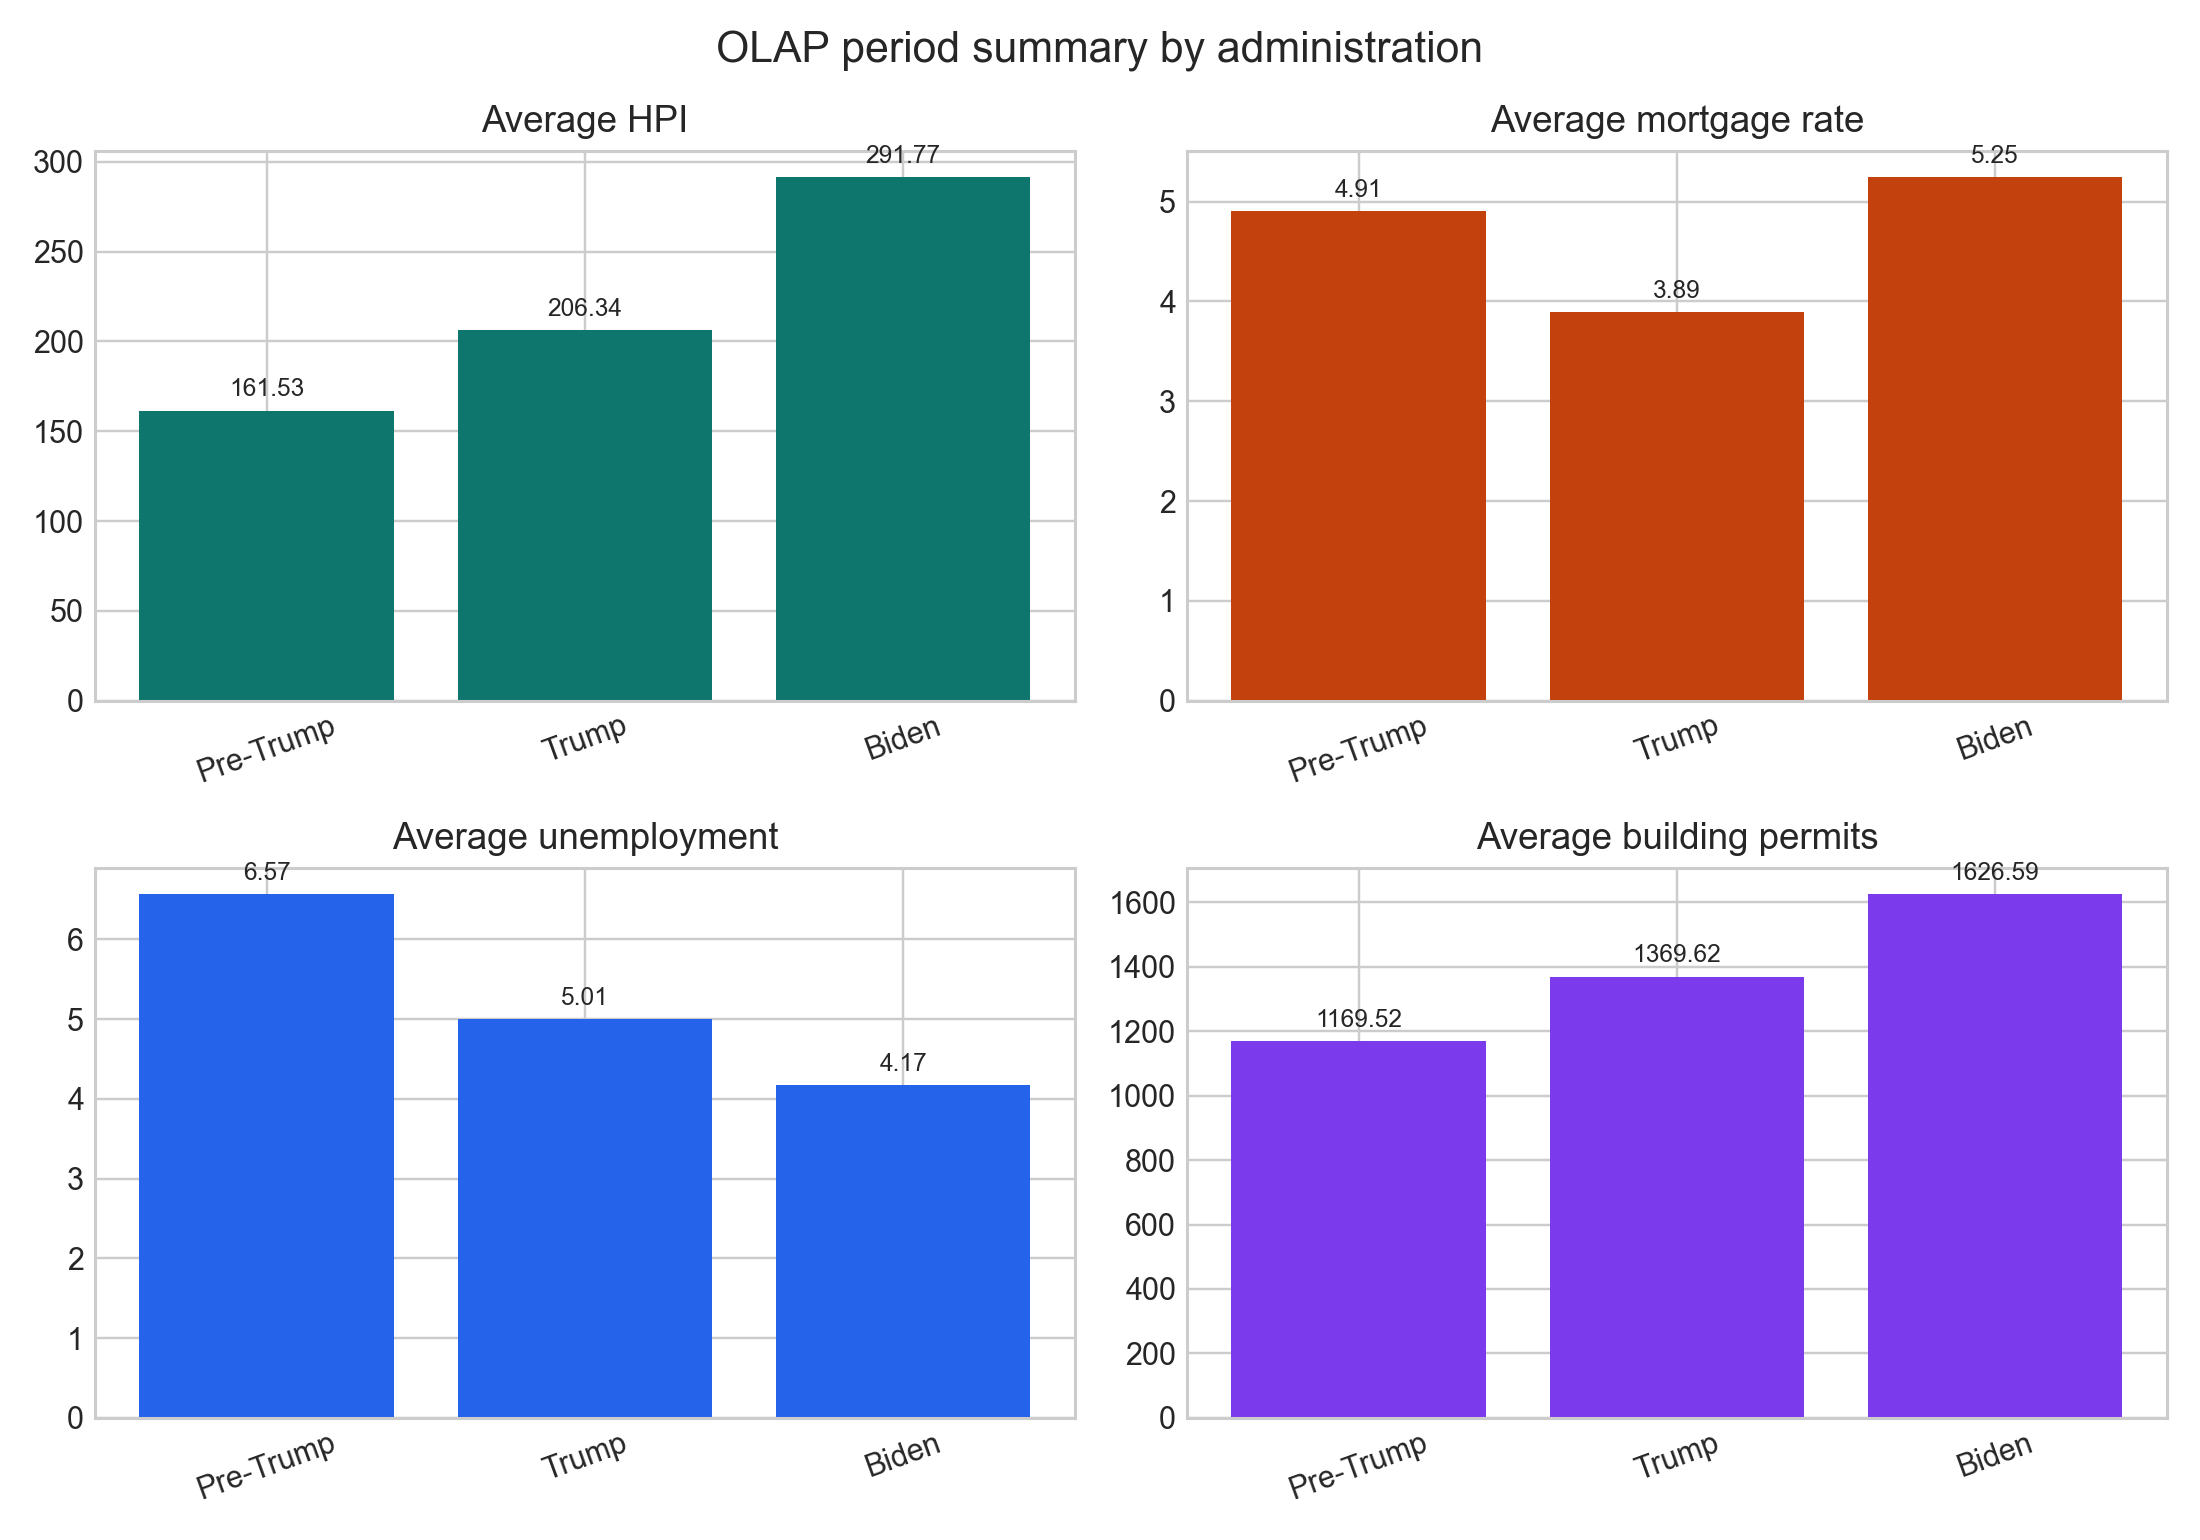
\includegraphics[width=0.95\textwidth]{figures/olap_period_results.png}
\caption{OLAP-style period comparison by administration.}
\label{fig:generated_olap}
\end{figure}

The OLAP summary shows that the highest average Home Price Index appears during the \textbf{Biden} period, while the highest average mortgage-rate pressure appears during the \textbf{Biden} period. This result is useful for the paper-review argument: prices and affordability pressure can rise together when supply, timing, and market inertia slow the response of prices.


\section{Limitations}

Despite the quality of the workflow, the project has several limitations.

First, the dataset may not capture all the determinants of housing prices.
Important factors such as regional heterogeneity, demographic evolution, or credit access variables may be absent.

Second, the forecasting logic is relatively simplified.
It uses a supervised learning strategy with lagged features rather than a dedicated time-series framework such as ARIMA, Prophet, or recurrent neural networks.

Third, the presented model results depend strongly on preprocessing decisions and the specific target selected by the user.
Different datasets or feature sets could lead to different outcomes.

\section{Recommendations and Future Improvements}

Several improvements can strengthen the project:
\begin{itemize}
\item integrate larger and more recent datasets,
\item include external APIs for automatic data refresh,
\item test advanced forecasting techniques,
\item improve the visual design of the dashboard,
\item add regional filtering or scenario analysis.
\end{itemize}

It would also be valuable to include a dedicated explainability module, for example with SHAP values, in order to deepen the interpretation of feature contributions.

\section{Conclusion}

This chapter discussed the most important results of the project.
The experiments showed that machine learning methods can provide useful insight into housing market dynamics and that Random Forest offers stronger predictive performance than Ridge Regression in the proposed setting.
At the same time, the dashboard contributed significantly to the interpretability and practical usability of the project.
Overall, the work confirms the relevance of data mining and machine learning for economic analysis and opens the door to more advanced future developments.

\section{Results from the Analytical Platform}

The platform produces a broad set of results that includes exploratory findings, Ridge Regression, Random Forest, forecasting, comparative model evaluation, unsupervised discovery, OLAP summaries, reinforcement-learning interpretation, paper review, production-readiness checks, and business impact analysis.

\section{Supervised Model Comparison}

The expanded model laboratory makes it possible to compare different algorithms on the same dataset and feature selection. This improves the reliability of the modeling decision. A model should not be selected only because it is popular; it should be selected because it performs well, remains interpretable enough for the context, and behaves consistently.

\begin{longtable}{p{4cm}p{5cm}p{5cm}}
\toprule
\textbf{Model family} & \textbf{Strength} & \textbf{Limitation} \\
\midrule
Linear Regression & Simple and interpretable & May underfit non-linear relationships. \\
Ridge Regression & Stable baseline with regularization & Still mainly linear. \\
Random Forest & Captures non-linear patterns and interactions & Less transparent than linear models. \\
Gradient Boosting & Often strong predictive accuracy & Requires careful tuning. \\
Decision Tree & Easy to visualize conceptually & Can overfit without constraints. \\
Support Vector Regression & Effective for complex boundaries & Sensitive to scaling and parameters. \\
KNN & Simple similarity-based logic & Can be weak in high dimensions. \\
Neural Network & Flexible function approximation & Requires more data and careful training. \\
\bottomrule
\caption{Interpretation of model families used in the platform.}
\end{longtable}

\section{Interpretation of Unsupervised Results}

The unsupervised learning results should be interpreted as exploratory findings. Clusters do not automatically represent economic truth; they identify similarity patterns according to selected features. If clusters align with known historical periods, this strengthens the interpretation. If clusters cut across periods, this suggests that macroeconomic profiles may be more complex than political labels alone.

PCA helps identify whether a small number of components explain much of the variation in the dataset. If the first two components explain a large share of the variance, visual analysis becomes more reliable. If the explained variance is low, the dataset is more complex and cannot be summarized easily in two dimensions.

Anomaly detection is particularly useful for housing-market analysis because abnormal periods can correspond to major economic shocks. These may include the financial crisis, pandemic-related disruptions, or high-rate affordability pressure.

\section{OLAP Results and Interpretation}

OLAP summaries provide a bridge between raw data and business understanding. For example, grouping indicators by administration period can reveal whether average mortgage rates, unemployment, inflation, or housing prices differed strongly across periods. Pivot tables can also show how indicators behave across time segments.

The strength of OLAP is that it is easy to explain. A manager or non-technical user can understand averages, medians, and period comparisons more easily than complex model internals. For this reason, OLAP results are useful before and after machine learning. Before modeling, they help understand the data. After modeling, they help interpret whether model results are coherent with descriptive patterns.

\section{AI Chatbot Results}

The chatbot improves the accessibility of the project. Instead of requiring users to navigate every technical page alone, the AI assistant can explain metrics, summarize outputs, and guide the user through the dashboard. This is especially valuable in an academic project because it demonstrates awareness of user experience.

The chatbot should be used carefully. It should explain results based on the available data and avoid presenting predictions as certainty. Good chatbot behavior must include cautious language, context, and explanation of limitations.

\section{Paper Review and Theory Comparison}

The paper review and comparison module adds academic depth. A project about housing prices should not only show charts and models; it should also discuss whether the findings are consistent with economic theory.

The main theoretical expectations are:
\begin{itemize}
\item higher mortgage or interest rates generally reduce affordability and pressure prices downward;
\item higher unemployment can weaken demand;
\item stronger income can support demand;
\item limited supply can keep prices high even when affordability worsens;
\item housing prices often react slowly because real estate markets are less liquid than financial markets.
\end{itemize}

The project therefore compares observed correlations and period changes with these expectations. When the dataset supports theory, the conclusion becomes stronger. When it challenges theory, the result is still useful because it may reveal timing effects, omitted variables, or mixed market forces.

\section{Real-Market Period Comparison}

The system compares the dataset with major housing-market periods:
\begin{itemize}
\item pre-crisis housing boom,
\item financial-crisis correction,
\item recovery and expansion,
\item pandemic-era demand shock,
\item high-rate affordability pressure.
\end{itemize}

This period comparison is important because housing-market behavior cannot be understood only through one global correlation. A variable may have one effect during a normal period and another effect during a crisis period. The project therefore interprets the housing market as a dynamic system.

\section{Production-Readiness Results}

The production-readiness module evaluates whether the data and model environment are reliable enough for serious use. It checks conditions such as dataset availability, duplicates, missingness, date column detection, and target variable availability.

The purpose of this module is not to claim that the academic project is already an industrial product. Instead, it shows what would be required to move toward professional deployment. This includes monitoring, documentation, validation, and governance.

\section{Business Impact}

The business impact of the project can be summarized in three levels.

\subsection{Analytical Impact}

The platform helps users understand which indicators are associated with housing prices, how these indicators change over time, and how models use them for prediction.

\subsection{Decision-Support Impact}

The dashboard supports what-if thinking, model comparison, and scenario interpretation. This can help analysts prepare reports, explain risks, or discuss possible market directions.

\subsection{Educational Impact}

The project is also valuable as a learning platform. It demonstrates how several data science concepts connect in one real application: EDA, supervised learning, unsupervised learning, forecasting, OLAP, reinforcement learning, AI interaction, and deployment.

\section{Limitations}

The project remains subject to several limitations.

\begin{itemize}
\item The dataset may not include all relevant housing-market determinants.
\item National-level data can hide regional differences between states and cities.
\item Forecasting is based on supervised lag features and does not replace specialized econometric forecasting.
\item The reinforcement-learning module is educational and simplified.
\item Chatbot answers depend on prompt quality and available context.
\item Streamlit deployment is practical but still needs security, authentication, and monitoring for professional production.
\end{itemize}

\section{Recommendations}

Future improvements should include:
\begin{enumerate}
\item adding regional housing datasets,
\item connecting live APIs for economic indicators,
\item adding SHAP explainability,
\item improving chatbot grounding with retrieved dashboard results,
\item adding user authentication,
\item saving experiment history in a database,
\item deploying the app on a cloud platform,
\item creating automatic PDF report generation,
\item and comparing results with more academic papers.
\end{enumerate}

\section{General Discussion}

The project shows that useful data science is not only about obtaining the highest score. It is about creating a coherent analytical workflow. A strong model without interpretation is difficult to trust. A beautiful dashboard without validation is risky. A chatbot without data grounding can be misleading. For this reason, the platform combines several layers: data quality, visualization, modeling, evaluation, explanation, deployment, and governance.

This combination makes the project more realistic and more valuable. It reflects how modern data science products are expected to work in professional contexts.

\section{Conclusion of the Results}

The results confirm the relevance of data mining and machine learning for housing-market analysis. The system now provides not only predictions but also segmentation, comparison, explanation, and interactive assistance. The project therefore forms a broader housing intelligence platform with academic, technical, and business value.


\chapter*{General Conclusion and Future Work}
\label{chap:conclusion}
\markboth{\MakeUppercase{General Conclusion and Future Work}}{}%
\addcontentsline{toc}{chapter}{General Conclusion and Future Work}
This report presented a complete data mining and machine learning workflow for analyzing and predicting housing market behavior in the United States.
The work combined business understanding, exploratory data analysis, preprocessing, predictive modeling, dashboard design, and forecasting.
The results showed that macroeconomic indicators such as inflation, unemployment, and interest rates are strongly linked to housing market trends.
Among the tested models, Random Forest delivered stronger predictive performance, while Ridge Regression remained valuable because of its simplicity and interpretability.

The developed Streamlit dashboard also demonstrated the importance of interactive data visualization in supporting understanding and decision-making.
Although the project produced encouraging results, several improvements remain possible.
Future work may include adding larger datasets, using real-time data sources, testing advanced time-series models, and extending the dashboard with scenario simulation features.

The project integrates OLAP analysis, an AI chatbot, prompt-based interaction, unsupervised learning, reinforcement-learning simulation, experiment tracking, model registry logic, production-readiness validation, paper review, and business impact analysis. These components transform the dashboard into a complete housing intelligence platform.

The main lesson from the project is that a valuable data science solution must combine prediction, interpretation, usability, and governance. A model score alone is not enough. Users also need to understand the data, compare periods, test scenarios, detect hidden patterns, and interpret results in relation to real economic theory. The Streamlit application addresses these needs by connecting technical analysis with decision support.

Future work should focus on improving the chatbot grounding, adding regional housing datasets, integrating live economic APIs, implementing SHAP explainability, saving experiments in a persistent database, and deploying the application on a cloud platform. With these improvements, the project could become a stronger professional prototype for housing-market monitoring and economic decision support.

\bibliographystyle{plain}
\bibliography{Biblio}

\appendix
\chapter{Appendices}
\section{How to add your own screenshots}
Replace the example figures in this project with screenshots from your Streamlit dashboard exported as PNG or JPG.
Then adjust the filenames inside the corresponding figure environments.

\section{Main code excerpt}
The full Python application is included in this project package. Selected excerpts and running instructions are provided below.


\section{Application Files}

The project package includes the following important files:
\begin{itemize}
\item \texttt{streamlit\_app.py}: the main Streamlit application containing the complete analytical platform.
\item \texttt{us\_home\_price\_analysis\_2004\_2024.csv}: the dataset used by the project.
\end{itemize}

\section{Main Feature List from the Code}

The code includes modules for data cleaning and cleaning reports, dashboard navigation and custom theme, correlation summaries, supervised regression and classification, model evaluation across multiple algorithms, feature importance, forecasting with lags and rolling variables, theory checks, real-life market-period comparison, OLAP and export, unsupervised learning, reinforcement-learning simulation, AI chatbot and prompt-based interaction, experiment tracking, model registry, production-readiness validation, and business impact reporting.

\section{Selected Code Excerpt}

The following excerpt illustrates the type of model pipeline used in the application. The full source code is included in the ZIP package.

\begin{verbatim}
steps = [("imputer", SimpleImputer(strategy="median"))]
if use_scaling:
    scaler = StandardScaler() if scaler_name == "StandardScaler" else MinMaxScaler()
    steps.append(("scaler", scaler))
steps.append(("model", make_model(model_choice, task_type)))
pipeline = Pipeline(steps)
pipeline.fit(X_train, y_train)
predictions = pipeline.predict(X_test)
\end{verbatim}

\section{How to Run the Streamlit Application}

After installing the required Python packages, the application can be launched with:
\begin{verbatim}
streamlit run streamlit_app.py
\end{verbatim}

The dataset can be uploaded through the dashboard or placed in the expected data folder. The app then allows the user to explore, model, evaluate, forecast, export, and interpret the housing dataset.


\printglossaries
\printindex
\end{document}
